% =============================================================================
% 08-io-techniques.tex — Week 8: I/O Techniques (synchronous vs. asynchronous
% I/O; interrupts, polling, DMA, IOP)
%
% Course: Computer Organization and Architecture (PCC CS-401)
% Anchor reading: Hamacher Ch. 4 (I/O module, interrupts, DMA in the system
%                 bus context); Stallings Ch. 8 "Input/Output" in the 11th-ed.
%                 file on disk (confirmed via its own TOC 2026-08-11 --- NOT
%                 Ch. 7 as the syllabus assumes; see knowledge-base-CS401.md's
%                 edition-mismatch flag), sections 8.1-8.5 + 8.7: external
%                 devices, I/O modules, programmed I/O, interrupt-driven I/O,
%                 DMA, I/O channels/processors
%
% Running thread: getting bytes from a keyboard and blocks from a disk into a
% 1 GHz CPU's memory — quantifying the CPU cost of each I/O technique so the
% selected technique can be defended on latency/throughput grounds.
%
% Compile with: /compile-latex CS401/08-io-techniques
% =============================================================================

\documentclass[aspectratio=169]{beamer}
% =============================================================================
% Preambles/header.tex — shared LaTeX/Beamer preamble for this project
%
% Use from a Beamer lecture by prepending:
%     % =============================================================================
% Preambles/header.tex — shared LaTeX/Beamer preamble for this project
%
% Use from a Beamer lecture by prepending:
%     % =============================================================================
% Preambles/header.tex — shared LaTeX/Beamer preamble for this project
%
% Use from a Beamer lecture by prepending:
%     \input{header}
% and compiling with TEXINPUTS=../Preambles:$TEXINPUTS (the /compile-latex
% skill does this automatically).
%
% PALETTE CONTRACT. Color names defined here MUST match the names in
% Quarto/theme-template.scss so Beamer and Quarto renderings use the same
% palette. The scripts/check-palette-sync.sh script enforces this.
%
% To customize: edit the HEX values below AND the matching $variable in
% Quarto/theme-template.scss, then run scripts/check-palette-sync.sh.
%
% TITLE PAGE. A formal, serif (Libertine) title-page template is defined in
% the Beamer-only block below (\setbeamertemplate{title page}) -- title,
% subtitle, a thin gold rule, then \author/\institute/\date. Frametitle and
% body text remain on Beamer's sans-serif default. No SCSS counterpart is
% needed for this (font/layout only, no new colors).
% =============================================================================

% -----------------------------------------------------------------------------
% Engine detection + encoding
%
% Our /compile-latex skill uses XeLaTeX, where inputenc is unnecessary and
% can produce encoding warnings. Only load inputenc under pdfTeX.
% -----------------------------------------------------------------------------
\usepackage{iftex}
\ifPDFTeX
  \usepackage[utf8]{inputenc}
\fi

\usepackage{amsmath, amssymb, amsthm}
\usepackage{booktabs}
\usepackage{graphicx}

% -----------------------------------------------------------------------------
% Serif face for the title page (formal/academic look). Linux Libertine is
% XeLaTeX- and pdfTeX-safe and redefines \rmdefault, so \rmfamily picks it up
% everywhere \rmfamily is used explicitly. Body text and frametitles stay on
% Beamer's own sans-serif default (unaffected) -- only the title-page
% \setbeamerfont{...} overrides below opt in to \rmfamily.
% -----------------------------------------------------------------------------
\usepackage{libertine}

% -----------------------------------------------------------------------------
% PALETTE — mirrors Quarto/theme-template.scss variable names.
% Load xcolor and define colors BEFORE anything that references them
% (notably hyperref, hypersetup, and the Beamer color assignments).
% -----------------------------------------------------------------------------
\usepackage{xcolor}

\definecolor{primary-blue}{HTML}{012169}      % headings, accents
\definecolor{primary-gold}{HTML}{B9975B}      % emphasis, borders
\definecolor{highlight-yellow}{HTML}{F2A900}  % markers, alerts
\definecolor{light-bg}{HTML}{E8EDF5}          % title / section backgrounds
\definecolor{jet}{HTML}{1A1A1A}               % body text

% Semantic colors (used in diagrams and annotations)
\definecolor{positive}{HTML}{15803D}          % good / observed / identified
\definecolor{negative}{HTML}{B91C1C}          % bad / problematic / bias
\definecolor{neutral}{HTML}{525252}           % reference / context

% Highlight accents (match .hi-* classes in the SCSS)
\definecolor{hi-slate}{HTML}{314F4F}
\definecolor{hi-green}{HTML}{2E8B57}
\definecolor{hi-red}{HTML}{C41E3A}

% Semantic aliases so skill templates and snippets can write
% \textcolor{accent}{...} without hard-coding "primary-blue".
\colorlet{accent}{primary-blue}
\colorlet{accent2}{primary-gold}

% -----------------------------------------------------------------------------
% Hyperref — loaded AFTER xcolor + palette so link colors resolve.
% -----------------------------------------------------------------------------
\usepackage{hyperref}
\hypersetup{colorlinks=true, linkcolor=primary-blue, urlcolor=primary-blue,
            citecolor=primary-blue, pdfborder={0 0 0}}

% -----------------------------------------------------------------------------
% Course code — set once per deck (after \input{header}, before \begin{document})
% via \coursecode{CS401}. Shown in the footer on every slide so a deck's course
% is identifiable without opening the title page. Empty by default.
% -----------------------------------------------------------------------------
\makeatletter
\newcommand{\coursecode}[1]{\gdef\@coursecodetext{#1}}
\gdef\@coursecodetext{}
\makeatother

% -----------------------------------------------------------------------------
% Beamer theme assignments (only apply under Beamer).
%
% We detect Beamer via \@ifclassloaded{beamer}, which is the documented,
% non-internal way. This must be wrapped in \makeatletter/\makeatother
% because \@ifclassloaded contains an @-catcode character.
% -----------------------------------------------------------------------------
\makeatletter
\@ifclassloaded{beamer}{%
  \usefonttheme{professionalfonts}
  \setbeamercolor{structure}{fg=primary-blue}
  \setbeamercolor{frametitle}{fg=primary-blue}
  \setbeamercolor{title}{fg=primary-blue}
  \setbeamercolor{subtitle}{fg=primary-gold}
  \setbeamercolor{author}{fg=primary-blue}
  \setbeamercolor{institute}{fg=neutral}
  \setbeamercolor{date}{fg=primary-gold}
  \setbeamercolor{itemize item}{fg=primary-blue}
  \setbeamercolor{itemize subitem}{fg=primary-gold}
  \setbeamercolor{alerted text}{fg=primary-gold}
  \setbeamercolor{block title}{fg=white, bg=primary-blue}
  \setbeamercolor{block body}{bg=light-bg}
  % Semantic block variants: block=definition/concept (blue), exampleblock=
  % worked example (green/positive), alertblock=key takeaway or caution (gold).
  % Keep to <=2 colored boxes per slide across ALL three variants (INV-7).
  \setbeamercolor{block title example}{fg=white, bg=positive}
  \setbeamercolor{block body example}{bg=light-bg}
  \setbeamercolor{block title alerted}{fg=white, bg=primary-gold}
  \setbeamercolor{block body alerted}{bg=light-bg}

  % ---------------------------------------------------------------------------
  % Formal title page: serif (Libertine, via \rmfamily) for title-page
  % elements only. Body text, itemize, and frametitle are intentionally left
  % on Beamer's sans-serif default -- \usebeamerfont{title} is also what
  % \transitionslide (below) uses for its big centered text, so section
  % transitions pick up the same serif treatment for free.
  % ---------------------------------------------------------------------------
  \setbeamerfont{title}{family=\rmfamily, series=\bfseries, size=\Large}
  \setbeamerfont{subtitle}{family=\rmfamily, shape=\itshape, size=\normalsize}
  \setbeamerfont{author}{family=\rmfamily, size=\normalsize}
  \setbeamerfont{institute}{family=\rmfamily, size=\scriptsize}
  \setbeamerfont{date}{family=\rmfamily, size=\scriptsize}

  \setbeamertemplate{title page}{
    \vfill
    \begin{center}
      {\usebeamerfont{title}\usebeamercolor[fg]{title}\inserttitle\par}
      \vspace{0.15cm}
      {\usebeamerfont{subtitle}\usebeamercolor[fg]{subtitle}\insertsubtitle\par}
      \vspace{0.45cm}
      {\color{primary-gold}\rule{0.42\textwidth}{0.6pt}\par}
      \vspace{0.45cm}
      {\usebeamerfont{author}\usebeamercolor[fg]{author}\insertauthor\par}
      \vspace{0.35cm}
      {\usebeamerfont{institute}\usebeamercolor[fg]{institute}\insertinstitute\par}
      \vspace{0.35cm}
      {\usebeamerfont{date}\usebeamercolor[fg]{date}\insertdate\par}
    \end{center}
    \vfill
  }

  % Minimal footer: course code (left) + page X / N (right), no navigation clutter
  \setbeamertemplate{navigation symbols}{}
  \setbeamertemplate{footline}{%
    \color{neutral}\footnotesize\hspace{0.7em}\@coursecodetext\hfill
    \insertframenumber/\inserttotalframenumber\hspace{0.7em}\vspace{0.3em}}
}{}
\makeatother

% -----------------------------------------------------------------------------
% TikZ setup — libraries the snippet gallery uses
% -----------------------------------------------------------------------------
\usepackage{tikz}
\usetikzlibrary{arrows.meta, positioning, calc, decorations.pathreplacing,
                fit, shapes.geometric, backgrounds}

% Shared TikZ styles — snippets and hand-written diagrams can pick these up
% via `\begin{tikzpicture}[every node/.style={...}]` or by naming specific
% styles (e.g., `\node[dag-node] (X) at (0,0) {X};`).
\tikzset{
  % Node styles for causal DAGs and similar
  dag-node/.style = {
    draw=primary-blue, fill=light-bg, rounded corners=2pt,
    minimum width=1.2cm, minimum height=0.9cm, align=center, font=\small
  },
  decision-node/.style = {
    draw=primary-gold, fill=white, diamond, aspect=1.8,
    minimum width=1.8cm, minimum height=1.2cm, align=center, font=\small,
    inner sep=1pt
  },
  % Edge styles — observed vs counterfactual
  observed-edge/.style = {-{Latex[length=2.5mm]}, thick, draw=jet},
  counterfactual-edge/.style = {-{Latex[length=2.5mm]}, thick, draw=neutral, dashed},
  confound-edge/.style = {-{Latex[length=2.5mm]}, thick, draw=negative, dashed},
  % Data-point styles for plots
  observed-dot/.style = {fill=primary-blue, draw=primary-blue, circle, inner sep=1.2pt},
  counterfactual-dot/.style = {fill=white, draw=neutral, circle, inner sep=1.2pt}
}

% -----------------------------------------------------------------------------
% Convenience macros
% -----------------------------------------------------------------------------
\newcommand{\muted}[1]{\textcolor{neutral}{#1}}
\newcommand{\key}[1]{\textcolor{primary-gold}{\textbf{#1}}}
\newcommand{\good}[1]{\textcolor{positive}{#1}}
\newcommand{\bad}[1]{\textcolor{negative}{#1}}

% Standout frame macro: full-bleed dark background for section transitions.
% Beamer-only (uses \begin{frame}/\setbeamercolor/\usebeamerfont) -- do not
% call from an article-class file (e.g. Notes/<CODE>/*-notes.tex). \muted,
% \key, \good, \bad, and \coursecode above are plain xcolor/gdef and are
% safe to use from either class; verified when Notes/article-class support
% was added.
% Expand: \transitionslide{Your transition title}
\newcommand{\transitionslide}[1]{%
  \begingroup
  \setbeamercolor{background canvas}{bg=primary-blue}
  \begin{frame}[plain]
    \centering
    \vfill
    {\usebeamerfont{title}\color{white}\Large #1\par}
    \vfill
  \end{frame}
  \endgroup
}

% and compiling with TEXINPUTS=../Preambles:$TEXINPUTS (the /compile-latex
% skill does this automatically).
%
% PALETTE CONTRACT. Color names defined here MUST match the names in
% Quarto/theme-template.scss so Beamer and Quarto renderings use the same
% palette. The scripts/check-palette-sync.sh script enforces this.
%
% To customize: edit the HEX values below AND the matching $variable in
% Quarto/theme-template.scss, then run scripts/check-palette-sync.sh.
%
% TITLE PAGE. A formal, serif (Libertine) title-page template is defined in
% the Beamer-only block below (\setbeamertemplate{title page}) -- title,
% subtitle, a thin gold rule, then \author/\institute/\date. Frametitle and
% body text remain on Beamer's sans-serif default. No SCSS counterpart is
% needed for this (font/layout only, no new colors).
% =============================================================================

% -----------------------------------------------------------------------------
% Engine detection + encoding
%
% Our /compile-latex skill uses XeLaTeX, where inputenc is unnecessary and
% can produce encoding warnings. Only load inputenc under pdfTeX.
% -----------------------------------------------------------------------------
\usepackage{iftex}
\ifPDFTeX
  \usepackage[utf8]{inputenc}
\fi

\usepackage{amsmath, amssymb, amsthm}
\usepackage{booktabs}
\usepackage{graphicx}

% -----------------------------------------------------------------------------
% Serif face for the title page (formal/academic look). Linux Libertine is
% XeLaTeX- and pdfTeX-safe and redefines \rmdefault, so \rmfamily picks it up
% everywhere \rmfamily is used explicitly. Body text and frametitles stay on
% Beamer's own sans-serif default (unaffected) -- only the title-page
% \setbeamerfont{...} overrides below opt in to \rmfamily.
% -----------------------------------------------------------------------------
\usepackage{libertine}

% -----------------------------------------------------------------------------
% PALETTE — mirrors Quarto/theme-template.scss variable names.
% Load xcolor and define colors BEFORE anything that references them
% (notably hyperref, hypersetup, and the Beamer color assignments).
% -----------------------------------------------------------------------------
\usepackage{xcolor}

\definecolor{primary-blue}{HTML}{012169}      % headings, accents
\definecolor{primary-gold}{HTML}{B9975B}      % emphasis, borders
\definecolor{highlight-yellow}{HTML}{F2A900}  % markers, alerts
\definecolor{light-bg}{HTML}{E8EDF5}          % title / section backgrounds
\definecolor{jet}{HTML}{1A1A1A}               % body text

% Semantic colors (used in diagrams and annotations)
\definecolor{positive}{HTML}{15803D}          % good / observed / identified
\definecolor{negative}{HTML}{B91C1C}          % bad / problematic / bias
\definecolor{neutral}{HTML}{525252}           % reference / context

% Highlight accents (match .hi-* classes in the SCSS)
\definecolor{hi-slate}{HTML}{314F4F}
\definecolor{hi-green}{HTML}{2E8B57}
\definecolor{hi-red}{HTML}{C41E3A}

% Semantic aliases so skill templates and snippets can write
% \textcolor{accent}{...} without hard-coding "primary-blue".
\colorlet{accent}{primary-blue}
\colorlet{accent2}{primary-gold}

% -----------------------------------------------------------------------------
% Hyperref — loaded AFTER xcolor + palette so link colors resolve.
% -----------------------------------------------------------------------------
\usepackage{hyperref}
\hypersetup{colorlinks=true, linkcolor=primary-blue, urlcolor=primary-blue,
            citecolor=primary-blue, pdfborder={0 0 0}}

% -----------------------------------------------------------------------------
% Course code — set once per deck (after % =============================================================================
% Preambles/header.tex — shared LaTeX/Beamer preamble for this project
%
% Use from a Beamer lecture by prepending:
%     \input{header}
% and compiling with TEXINPUTS=../Preambles:$TEXINPUTS (the /compile-latex
% skill does this automatically).
%
% PALETTE CONTRACT. Color names defined here MUST match the names in
% Quarto/theme-template.scss so Beamer and Quarto renderings use the same
% palette. The scripts/check-palette-sync.sh script enforces this.
%
% To customize: edit the HEX values below AND the matching $variable in
% Quarto/theme-template.scss, then run scripts/check-palette-sync.sh.
%
% TITLE PAGE. A formal, serif (Libertine) title-page template is defined in
% the Beamer-only block below (\setbeamertemplate{title page}) -- title,
% subtitle, a thin gold rule, then \author/\institute/\date. Frametitle and
% body text remain on Beamer's sans-serif default. No SCSS counterpart is
% needed for this (font/layout only, no new colors).
% =============================================================================

% -----------------------------------------------------------------------------
% Engine detection + encoding
%
% Our /compile-latex skill uses XeLaTeX, where inputenc is unnecessary and
% can produce encoding warnings. Only load inputenc under pdfTeX.
% -----------------------------------------------------------------------------
\usepackage{iftex}
\ifPDFTeX
  \usepackage[utf8]{inputenc}
\fi

\usepackage{amsmath, amssymb, amsthm}
\usepackage{booktabs}
\usepackage{graphicx}

% -----------------------------------------------------------------------------
% Serif face for the title page (formal/academic look). Linux Libertine is
% XeLaTeX- and pdfTeX-safe and redefines \rmdefault, so \rmfamily picks it up
% everywhere \rmfamily is used explicitly. Body text and frametitles stay on
% Beamer's own sans-serif default (unaffected) -- only the title-page
% \setbeamerfont{...} overrides below opt in to \rmfamily.
% -----------------------------------------------------------------------------
\usepackage{libertine}

% -----------------------------------------------------------------------------
% PALETTE — mirrors Quarto/theme-template.scss variable names.
% Load xcolor and define colors BEFORE anything that references them
% (notably hyperref, hypersetup, and the Beamer color assignments).
% -----------------------------------------------------------------------------
\usepackage{xcolor}

\definecolor{primary-blue}{HTML}{012169}      % headings, accents
\definecolor{primary-gold}{HTML}{B9975B}      % emphasis, borders
\definecolor{highlight-yellow}{HTML}{F2A900}  % markers, alerts
\definecolor{light-bg}{HTML}{E8EDF5}          % title / section backgrounds
\definecolor{jet}{HTML}{1A1A1A}               % body text

% Semantic colors (used in diagrams and annotations)
\definecolor{positive}{HTML}{15803D}          % good / observed / identified
\definecolor{negative}{HTML}{B91C1C}          % bad / problematic / bias
\definecolor{neutral}{HTML}{525252}           % reference / context

% Highlight accents (match .hi-* classes in the SCSS)
\definecolor{hi-slate}{HTML}{314F4F}
\definecolor{hi-green}{HTML}{2E8B57}
\definecolor{hi-red}{HTML}{C41E3A}

% Semantic aliases so skill templates and snippets can write
% \textcolor{accent}{...} without hard-coding "primary-blue".
\colorlet{accent}{primary-blue}
\colorlet{accent2}{primary-gold}

% -----------------------------------------------------------------------------
% Hyperref — loaded AFTER xcolor + palette so link colors resolve.
% -----------------------------------------------------------------------------
\usepackage{hyperref}
\hypersetup{colorlinks=true, linkcolor=primary-blue, urlcolor=primary-blue,
            citecolor=primary-blue, pdfborder={0 0 0}}

% -----------------------------------------------------------------------------
% Course code — set once per deck (after \input{header}, before \begin{document})
% via \coursecode{CS401}. Shown in the footer on every slide so a deck's course
% is identifiable without opening the title page. Empty by default.
% -----------------------------------------------------------------------------
\makeatletter
\newcommand{\coursecode}[1]{\gdef\@coursecodetext{#1}}
\gdef\@coursecodetext{}
\makeatother

% -----------------------------------------------------------------------------
% Beamer theme assignments (only apply under Beamer).
%
% We detect Beamer via \@ifclassloaded{beamer}, which is the documented,
% non-internal way. This must be wrapped in \makeatletter/\makeatother
% because \@ifclassloaded contains an @-catcode character.
% -----------------------------------------------------------------------------
\makeatletter
\@ifclassloaded{beamer}{%
  \usefonttheme{professionalfonts}
  \setbeamercolor{structure}{fg=primary-blue}
  \setbeamercolor{frametitle}{fg=primary-blue}
  \setbeamercolor{title}{fg=primary-blue}
  \setbeamercolor{subtitle}{fg=primary-gold}
  \setbeamercolor{author}{fg=primary-blue}
  \setbeamercolor{institute}{fg=neutral}
  \setbeamercolor{date}{fg=primary-gold}
  \setbeamercolor{itemize item}{fg=primary-blue}
  \setbeamercolor{itemize subitem}{fg=primary-gold}
  \setbeamercolor{alerted text}{fg=primary-gold}
  \setbeamercolor{block title}{fg=white, bg=primary-blue}
  \setbeamercolor{block body}{bg=light-bg}
  % Semantic block variants: block=definition/concept (blue), exampleblock=
  % worked example (green/positive), alertblock=key takeaway or caution (gold).
  % Keep to <=2 colored boxes per slide across ALL three variants (INV-7).
  \setbeamercolor{block title example}{fg=white, bg=positive}
  \setbeamercolor{block body example}{bg=light-bg}
  \setbeamercolor{block title alerted}{fg=white, bg=primary-gold}
  \setbeamercolor{block body alerted}{bg=light-bg}

  % ---------------------------------------------------------------------------
  % Formal title page: serif (Libertine, via \rmfamily) for title-page
  % elements only. Body text, itemize, and frametitle are intentionally left
  % on Beamer's sans-serif default -- \usebeamerfont{title} is also what
  % \transitionslide (below) uses for its big centered text, so section
  % transitions pick up the same serif treatment for free.
  % ---------------------------------------------------------------------------
  \setbeamerfont{title}{family=\rmfamily, series=\bfseries, size=\Large}
  \setbeamerfont{subtitle}{family=\rmfamily, shape=\itshape, size=\normalsize}
  \setbeamerfont{author}{family=\rmfamily, size=\normalsize}
  \setbeamerfont{institute}{family=\rmfamily, size=\scriptsize}
  \setbeamerfont{date}{family=\rmfamily, size=\scriptsize}

  \setbeamertemplate{title page}{
    \vfill
    \begin{center}
      {\usebeamerfont{title}\usebeamercolor[fg]{title}\inserttitle\par}
      \vspace{0.15cm}
      {\usebeamerfont{subtitle}\usebeamercolor[fg]{subtitle}\insertsubtitle\par}
      \vspace{0.45cm}
      {\color{primary-gold}\rule{0.42\textwidth}{0.6pt}\par}
      \vspace{0.45cm}
      {\usebeamerfont{author}\usebeamercolor[fg]{author}\insertauthor\par}
      \vspace{0.35cm}
      {\usebeamerfont{institute}\usebeamercolor[fg]{institute}\insertinstitute\par}
      \vspace{0.35cm}
      {\usebeamerfont{date}\usebeamercolor[fg]{date}\insertdate\par}
    \end{center}
    \vfill
  }

  % Minimal footer: course code (left) + page X / N (right), no navigation clutter
  \setbeamertemplate{navigation symbols}{}
  \setbeamertemplate{footline}{%
    \color{neutral}\footnotesize\hspace{0.7em}\@coursecodetext\hfill
    \insertframenumber/\inserttotalframenumber\hspace{0.7em}\vspace{0.3em}}
}{}
\makeatother

% -----------------------------------------------------------------------------
% TikZ setup — libraries the snippet gallery uses
% -----------------------------------------------------------------------------
\usepackage{tikz}
\usetikzlibrary{arrows.meta, positioning, calc, decorations.pathreplacing,
                fit, shapes.geometric, backgrounds}

% Shared TikZ styles — snippets and hand-written diagrams can pick these up
% via `\begin{tikzpicture}[every node/.style={...}]` or by naming specific
% styles (e.g., `\node[dag-node] (X) at (0,0) {X};`).
\tikzset{
  % Node styles for causal DAGs and similar
  dag-node/.style = {
    draw=primary-blue, fill=light-bg, rounded corners=2pt,
    minimum width=1.2cm, minimum height=0.9cm, align=center, font=\small
  },
  decision-node/.style = {
    draw=primary-gold, fill=white, diamond, aspect=1.8,
    minimum width=1.8cm, minimum height=1.2cm, align=center, font=\small,
    inner sep=1pt
  },
  % Edge styles — observed vs counterfactual
  observed-edge/.style = {-{Latex[length=2.5mm]}, thick, draw=jet},
  counterfactual-edge/.style = {-{Latex[length=2.5mm]}, thick, draw=neutral, dashed},
  confound-edge/.style = {-{Latex[length=2.5mm]}, thick, draw=negative, dashed},
  % Data-point styles for plots
  observed-dot/.style = {fill=primary-blue, draw=primary-blue, circle, inner sep=1.2pt},
  counterfactual-dot/.style = {fill=white, draw=neutral, circle, inner sep=1.2pt}
}

% -----------------------------------------------------------------------------
% Convenience macros
% -----------------------------------------------------------------------------
\newcommand{\muted}[1]{\textcolor{neutral}{#1}}
\newcommand{\key}[1]{\textcolor{primary-gold}{\textbf{#1}}}
\newcommand{\good}[1]{\textcolor{positive}{#1}}
\newcommand{\bad}[1]{\textcolor{negative}{#1}}

% Standout frame macro: full-bleed dark background for section transitions.
% Beamer-only (uses \begin{frame}/\setbeamercolor/\usebeamerfont) -- do not
% call from an article-class file (e.g. Notes/<CODE>/*-notes.tex). \muted,
% \key, \good, \bad, and \coursecode above are plain xcolor/gdef and are
% safe to use from either class; verified when Notes/article-class support
% was added.
% Expand: \transitionslide{Your transition title}
\newcommand{\transitionslide}[1]{%
  \begingroup
  \setbeamercolor{background canvas}{bg=primary-blue}
  \begin{frame}[plain]
    \centering
    \vfill
    {\usebeamerfont{title}\color{white}\Large #1\par}
    \vfill
  \end{frame}
  \endgroup
}
, before \begin{document})
% via \coursecode{CS401}. Shown in the footer on every slide so a deck's course
% is identifiable without opening the title page. Empty by default.
% -----------------------------------------------------------------------------
\makeatletter
\newcommand{\coursecode}[1]{\gdef\@coursecodetext{#1}}
\gdef\@coursecodetext{}
\makeatother

% -----------------------------------------------------------------------------
% Beamer theme assignments (only apply under Beamer).
%
% We detect Beamer via \@ifclassloaded{beamer}, which is the documented,
% non-internal way. This must be wrapped in \makeatletter/\makeatother
% because \@ifclassloaded contains an @-catcode character.
% -----------------------------------------------------------------------------
\makeatletter
\@ifclassloaded{beamer}{%
  \usefonttheme{professionalfonts}
  \setbeamercolor{structure}{fg=primary-blue}
  \setbeamercolor{frametitle}{fg=primary-blue}
  \setbeamercolor{title}{fg=primary-blue}
  \setbeamercolor{subtitle}{fg=primary-gold}
  \setbeamercolor{author}{fg=primary-blue}
  \setbeamercolor{institute}{fg=neutral}
  \setbeamercolor{date}{fg=primary-gold}
  \setbeamercolor{itemize item}{fg=primary-blue}
  \setbeamercolor{itemize subitem}{fg=primary-gold}
  \setbeamercolor{alerted text}{fg=primary-gold}
  \setbeamercolor{block title}{fg=white, bg=primary-blue}
  \setbeamercolor{block body}{bg=light-bg}
  % Semantic block variants: block=definition/concept (blue), exampleblock=
  % worked example (green/positive), alertblock=key takeaway or caution (gold).
  % Keep to <=2 colored boxes per slide across ALL three variants (INV-7).
  \setbeamercolor{block title example}{fg=white, bg=positive}
  \setbeamercolor{block body example}{bg=light-bg}
  \setbeamercolor{block title alerted}{fg=white, bg=primary-gold}
  \setbeamercolor{block body alerted}{bg=light-bg}

  % ---------------------------------------------------------------------------
  % Formal title page: serif (Libertine, via \rmfamily) for title-page
  % elements only. Body text, itemize, and frametitle are intentionally left
  % on Beamer's sans-serif default -- \usebeamerfont{title} is also what
  % \transitionslide (below) uses for its big centered text, so section
  % transitions pick up the same serif treatment for free.
  % ---------------------------------------------------------------------------
  \setbeamerfont{title}{family=\rmfamily, series=\bfseries, size=\Large}
  \setbeamerfont{subtitle}{family=\rmfamily, shape=\itshape, size=\normalsize}
  \setbeamerfont{author}{family=\rmfamily, size=\normalsize}
  \setbeamerfont{institute}{family=\rmfamily, size=\scriptsize}
  \setbeamerfont{date}{family=\rmfamily, size=\scriptsize}

  \setbeamertemplate{title page}{
    \vfill
    \begin{center}
      {\usebeamerfont{title}\usebeamercolor[fg]{title}\inserttitle\par}
      \vspace{0.15cm}
      {\usebeamerfont{subtitle}\usebeamercolor[fg]{subtitle}\insertsubtitle\par}
      \vspace{0.45cm}
      {\color{primary-gold}\rule{0.42\textwidth}{0.6pt}\par}
      \vspace{0.45cm}
      {\usebeamerfont{author}\usebeamercolor[fg]{author}\insertauthor\par}
      \vspace{0.35cm}
      {\usebeamerfont{institute}\usebeamercolor[fg]{institute}\insertinstitute\par}
      \vspace{0.35cm}
      {\usebeamerfont{date}\usebeamercolor[fg]{date}\insertdate\par}
    \end{center}
    \vfill
  }

  % Minimal footer: course code (left) + page X / N (right), no navigation clutter
  \setbeamertemplate{navigation symbols}{}
  \setbeamertemplate{footline}{%
    \color{neutral}\footnotesize\hspace{0.7em}\@coursecodetext\hfill
    \insertframenumber/\inserttotalframenumber\hspace{0.7em}\vspace{0.3em}}
}{}
\makeatother

% -----------------------------------------------------------------------------
% TikZ setup — libraries the snippet gallery uses
% -----------------------------------------------------------------------------
\usepackage{tikz}
\usetikzlibrary{arrows.meta, positioning, calc, decorations.pathreplacing,
                fit, shapes.geometric, backgrounds}

% Shared TikZ styles — snippets and hand-written diagrams can pick these up
% via `\begin{tikzpicture}[every node/.style={...}]` or by naming specific
% styles (e.g., `\node[dag-node] (X) at (0,0) {X};`).
\tikzset{
  % Node styles for causal DAGs and similar
  dag-node/.style = {
    draw=primary-blue, fill=light-bg, rounded corners=2pt,
    minimum width=1.2cm, minimum height=0.9cm, align=center, font=\small
  },
  decision-node/.style = {
    draw=primary-gold, fill=white, diamond, aspect=1.8,
    minimum width=1.8cm, minimum height=1.2cm, align=center, font=\small,
    inner sep=1pt
  },
  % Edge styles — observed vs counterfactual
  observed-edge/.style = {-{Latex[length=2.5mm]}, thick, draw=jet},
  counterfactual-edge/.style = {-{Latex[length=2.5mm]}, thick, draw=neutral, dashed},
  confound-edge/.style = {-{Latex[length=2.5mm]}, thick, draw=negative, dashed},
  % Data-point styles for plots
  observed-dot/.style = {fill=primary-blue, draw=primary-blue, circle, inner sep=1.2pt},
  counterfactual-dot/.style = {fill=white, draw=neutral, circle, inner sep=1.2pt}
}

% -----------------------------------------------------------------------------
% Convenience macros
% -----------------------------------------------------------------------------
\newcommand{\muted}[1]{\textcolor{neutral}{#1}}
\newcommand{\key}[1]{\textcolor{primary-gold}{\textbf{#1}}}
\newcommand{\good}[1]{\textcolor{positive}{#1}}
\newcommand{\bad}[1]{\textcolor{negative}{#1}}

% Standout frame macro: full-bleed dark background for section transitions.
% Beamer-only (uses \begin{frame}/\setbeamercolor/\usebeamerfont) -- do not
% call from an article-class file (e.g. Notes/<CODE>/*-notes.tex). \muted,
% \key, \good, \bad, and \coursecode above are plain xcolor/gdef and are
% safe to use from either class; verified when Notes/article-class support
% was added.
% Expand: \transitionslide{Your transition title}
\newcommand{\transitionslide}[1]{%
  \begingroup
  \setbeamercolor{background canvas}{bg=primary-blue}
  \begin{frame}[plain]
    \centering
    \vfill
    {\usebeamerfont{title}\color{white}\Large #1\par}
    \vfill
  \end{frame}
  \endgroup
}

% and compiling with TEXINPUTS=../Preambles:$TEXINPUTS (the /compile-latex
% skill does this automatically).
%
% PALETTE CONTRACT. Color names defined here MUST match the names in
% Quarto/theme-template.scss so Beamer and Quarto renderings use the same
% palette. The scripts/check-palette-sync.sh script enforces this.
%
% To customize: edit the HEX values below AND the matching $variable in
% Quarto/theme-template.scss, then run scripts/check-palette-sync.sh.
%
% TITLE PAGE. A formal, serif (Libertine) title-page template is defined in
% the Beamer-only block below (\setbeamertemplate{title page}) -- title,
% subtitle, a thin gold rule, then \author/\institute/\date. Frametitle and
% body text remain on Beamer's sans-serif default. No SCSS counterpart is
% needed for this (font/layout only, no new colors).
% =============================================================================

% -----------------------------------------------------------------------------
% Engine detection + encoding
%
% Our /compile-latex skill uses XeLaTeX, where inputenc is unnecessary and
% can produce encoding warnings. Only load inputenc under pdfTeX.
% -----------------------------------------------------------------------------
\usepackage{iftex}
\ifPDFTeX
  \usepackage[utf8]{inputenc}
\fi

\usepackage{amsmath, amssymb, amsthm}
\usepackage{booktabs}
\usepackage{graphicx}

% -----------------------------------------------------------------------------
% Serif face for the title page (formal/academic look). Linux Libertine is
% XeLaTeX- and pdfTeX-safe and redefines \rmdefault, so \rmfamily picks it up
% everywhere \rmfamily is used explicitly. Body text and frametitles stay on
% Beamer's own sans-serif default (unaffected) -- only the title-page
% \setbeamerfont{...} overrides below opt in to \rmfamily.
% -----------------------------------------------------------------------------
\usepackage{libertine}

% -----------------------------------------------------------------------------
% PALETTE — mirrors Quarto/theme-template.scss variable names.
% Load xcolor and define colors BEFORE anything that references them
% (notably hyperref, hypersetup, and the Beamer color assignments).
% -----------------------------------------------------------------------------
\usepackage{xcolor}

\definecolor{primary-blue}{HTML}{012169}      % headings, accents
\definecolor{primary-gold}{HTML}{B9975B}      % emphasis, borders
\definecolor{highlight-yellow}{HTML}{F2A900}  % markers, alerts
\definecolor{light-bg}{HTML}{E8EDF5}          % title / section backgrounds
\definecolor{jet}{HTML}{1A1A1A}               % body text

% Semantic colors (used in diagrams and annotations)
\definecolor{positive}{HTML}{15803D}          % good / observed / identified
\definecolor{negative}{HTML}{B91C1C}          % bad / problematic / bias
\definecolor{neutral}{HTML}{525252}           % reference / context

% Highlight accents (match .hi-* classes in the SCSS)
\definecolor{hi-slate}{HTML}{314F4F}
\definecolor{hi-green}{HTML}{2E8B57}
\definecolor{hi-red}{HTML}{C41E3A}

% Semantic aliases so skill templates and snippets can write
% \textcolor{accent}{...} without hard-coding "primary-blue".
\colorlet{accent}{primary-blue}
\colorlet{accent2}{primary-gold}

% -----------------------------------------------------------------------------
% Hyperref — loaded AFTER xcolor + palette so link colors resolve.
% -----------------------------------------------------------------------------
\usepackage{hyperref}
\hypersetup{colorlinks=true, linkcolor=primary-blue, urlcolor=primary-blue,
            citecolor=primary-blue, pdfborder={0 0 0}}

% -----------------------------------------------------------------------------
% Course code — set once per deck (after % =============================================================================
% Preambles/header.tex — shared LaTeX/Beamer preamble for this project
%
% Use from a Beamer lecture by prepending:
%     % =============================================================================
% Preambles/header.tex — shared LaTeX/Beamer preamble for this project
%
% Use from a Beamer lecture by prepending:
%     \input{header}
% and compiling with TEXINPUTS=../Preambles:$TEXINPUTS (the /compile-latex
% skill does this automatically).
%
% PALETTE CONTRACT. Color names defined here MUST match the names in
% Quarto/theme-template.scss so Beamer and Quarto renderings use the same
% palette. The scripts/check-palette-sync.sh script enforces this.
%
% To customize: edit the HEX values below AND the matching $variable in
% Quarto/theme-template.scss, then run scripts/check-palette-sync.sh.
%
% TITLE PAGE. A formal, serif (Libertine) title-page template is defined in
% the Beamer-only block below (\setbeamertemplate{title page}) -- title,
% subtitle, a thin gold rule, then \author/\institute/\date. Frametitle and
% body text remain on Beamer's sans-serif default. No SCSS counterpart is
% needed for this (font/layout only, no new colors).
% =============================================================================

% -----------------------------------------------------------------------------
% Engine detection + encoding
%
% Our /compile-latex skill uses XeLaTeX, where inputenc is unnecessary and
% can produce encoding warnings. Only load inputenc under pdfTeX.
% -----------------------------------------------------------------------------
\usepackage{iftex}
\ifPDFTeX
  \usepackage[utf8]{inputenc}
\fi

\usepackage{amsmath, amssymb, amsthm}
\usepackage{booktabs}
\usepackage{graphicx}

% -----------------------------------------------------------------------------
% Serif face for the title page (formal/academic look). Linux Libertine is
% XeLaTeX- and pdfTeX-safe and redefines \rmdefault, so \rmfamily picks it up
% everywhere \rmfamily is used explicitly. Body text and frametitles stay on
% Beamer's own sans-serif default (unaffected) -- only the title-page
% \setbeamerfont{...} overrides below opt in to \rmfamily.
% -----------------------------------------------------------------------------
\usepackage{libertine}

% -----------------------------------------------------------------------------
% PALETTE — mirrors Quarto/theme-template.scss variable names.
% Load xcolor and define colors BEFORE anything that references them
% (notably hyperref, hypersetup, and the Beamer color assignments).
% -----------------------------------------------------------------------------
\usepackage{xcolor}

\definecolor{primary-blue}{HTML}{012169}      % headings, accents
\definecolor{primary-gold}{HTML}{B9975B}      % emphasis, borders
\definecolor{highlight-yellow}{HTML}{F2A900}  % markers, alerts
\definecolor{light-bg}{HTML}{E8EDF5}          % title / section backgrounds
\definecolor{jet}{HTML}{1A1A1A}               % body text

% Semantic colors (used in diagrams and annotations)
\definecolor{positive}{HTML}{15803D}          % good / observed / identified
\definecolor{negative}{HTML}{B91C1C}          % bad / problematic / bias
\definecolor{neutral}{HTML}{525252}           % reference / context

% Highlight accents (match .hi-* classes in the SCSS)
\definecolor{hi-slate}{HTML}{314F4F}
\definecolor{hi-green}{HTML}{2E8B57}
\definecolor{hi-red}{HTML}{C41E3A}

% Semantic aliases so skill templates and snippets can write
% \textcolor{accent}{...} without hard-coding "primary-blue".
\colorlet{accent}{primary-blue}
\colorlet{accent2}{primary-gold}

% -----------------------------------------------------------------------------
% Hyperref — loaded AFTER xcolor + palette so link colors resolve.
% -----------------------------------------------------------------------------
\usepackage{hyperref}
\hypersetup{colorlinks=true, linkcolor=primary-blue, urlcolor=primary-blue,
            citecolor=primary-blue, pdfborder={0 0 0}}

% -----------------------------------------------------------------------------
% Course code — set once per deck (after \input{header}, before \begin{document})
% via \coursecode{CS401}. Shown in the footer on every slide so a deck's course
% is identifiable without opening the title page. Empty by default.
% -----------------------------------------------------------------------------
\makeatletter
\newcommand{\coursecode}[1]{\gdef\@coursecodetext{#1}}
\gdef\@coursecodetext{}
\makeatother

% -----------------------------------------------------------------------------
% Beamer theme assignments (only apply under Beamer).
%
% We detect Beamer via \@ifclassloaded{beamer}, which is the documented,
% non-internal way. This must be wrapped in \makeatletter/\makeatother
% because \@ifclassloaded contains an @-catcode character.
% -----------------------------------------------------------------------------
\makeatletter
\@ifclassloaded{beamer}{%
  \usefonttheme{professionalfonts}
  \setbeamercolor{structure}{fg=primary-blue}
  \setbeamercolor{frametitle}{fg=primary-blue}
  \setbeamercolor{title}{fg=primary-blue}
  \setbeamercolor{subtitle}{fg=primary-gold}
  \setbeamercolor{author}{fg=primary-blue}
  \setbeamercolor{institute}{fg=neutral}
  \setbeamercolor{date}{fg=primary-gold}
  \setbeamercolor{itemize item}{fg=primary-blue}
  \setbeamercolor{itemize subitem}{fg=primary-gold}
  \setbeamercolor{alerted text}{fg=primary-gold}
  \setbeamercolor{block title}{fg=white, bg=primary-blue}
  \setbeamercolor{block body}{bg=light-bg}
  % Semantic block variants: block=definition/concept (blue), exampleblock=
  % worked example (green/positive), alertblock=key takeaway or caution (gold).
  % Keep to <=2 colored boxes per slide across ALL three variants (INV-7).
  \setbeamercolor{block title example}{fg=white, bg=positive}
  \setbeamercolor{block body example}{bg=light-bg}
  \setbeamercolor{block title alerted}{fg=white, bg=primary-gold}
  \setbeamercolor{block body alerted}{bg=light-bg}

  % ---------------------------------------------------------------------------
  % Formal title page: serif (Libertine, via \rmfamily) for title-page
  % elements only. Body text, itemize, and frametitle are intentionally left
  % on Beamer's sans-serif default -- \usebeamerfont{title} is also what
  % \transitionslide (below) uses for its big centered text, so section
  % transitions pick up the same serif treatment for free.
  % ---------------------------------------------------------------------------
  \setbeamerfont{title}{family=\rmfamily, series=\bfseries, size=\Large}
  \setbeamerfont{subtitle}{family=\rmfamily, shape=\itshape, size=\normalsize}
  \setbeamerfont{author}{family=\rmfamily, size=\normalsize}
  \setbeamerfont{institute}{family=\rmfamily, size=\scriptsize}
  \setbeamerfont{date}{family=\rmfamily, size=\scriptsize}

  \setbeamertemplate{title page}{
    \vfill
    \begin{center}
      {\usebeamerfont{title}\usebeamercolor[fg]{title}\inserttitle\par}
      \vspace{0.15cm}
      {\usebeamerfont{subtitle}\usebeamercolor[fg]{subtitle}\insertsubtitle\par}
      \vspace{0.45cm}
      {\color{primary-gold}\rule{0.42\textwidth}{0.6pt}\par}
      \vspace{0.45cm}
      {\usebeamerfont{author}\usebeamercolor[fg]{author}\insertauthor\par}
      \vspace{0.35cm}
      {\usebeamerfont{institute}\usebeamercolor[fg]{institute}\insertinstitute\par}
      \vspace{0.35cm}
      {\usebeamerfont{date}\usebeamercolor[fg]{date}\insertdate\par}
    \end{center}
    \vfill
  }

  % Minimal footer: course code (left) + page X / N (right), no navigation clutter
  \setbeamertemplate{navigation symbols}{}
  \setbeamertemplate{footline}{%
    \color{neutral}\footnotesize\hspace{0.7em}\@coursecodetext\hfill
    \insertframenumber/\inserttotalframenumber\hspace{0.7em}\vspace{0.3em}}
}{}
\makeatother

% -----------------------------------------------------------------------------
% TikZ setup — libraries the snippet gallery uses
% -----------------------------------------------------------------------------
\usepackage{tikz}
\usetikzlibrary{arrows.meta, positioning, calc, decorations.pathreplacing,
                fit, shapes.geometric, backgrounds}

% Shared TikZ styles — snippets and hand-written diagrams can pick these up
% via `\begin{tikzpicture}[every node/.style={...}]` or by naming specific
% styles (e.g., `\node[dag-node] (X) at (0,0) {X};`).
\tikzset{
  % Node styles for causal DAGs and similar
  dag-node/.style = {
    draw=primary-blue, fill=light-bg, rounded corners=2pt,
    minimum width=1.2cm, minimum height=0.9cm, align=center, font=\small
  },
  decision-node/.style = {
    draw=primary-gold, fill=white, diamond, aspect=1.8,
    minimum width=1.8cm, minimum height=1.2cm, align=center, font=\small,
    inner sep=1pt
  },
  % Edge styles — observed vs counterfactual
  observed-edge/.style = {-{Latex[length=2.5mm]}, thick, draw=jet},
  counterfactual-edge/.style = {-{Latex[length=2.5mm]}, thick, draw=neutral, dashed},
  confound-edge/.style = {-{Latex[length=2.5mm]}, thick, draw=negative, dashed},
  % Data-point styles for plots
  observed-dot/.style = {fill=primary-blue, draw=primary-blue, circle, inner sep=1.2pt},
  counterfactual-dot/.style = {fill=white, draw=neutral, circle, inner sep=1.2pt}
}

% -----------------------------------------------------------------------------
% Convenience macros
% -----------------------------------------------------------------------------
\newcommand{\muted}[1]{\textcolor{neutral}{#1}}
\newcommand{\key}[1]{\textcolor{primary-gold}{\textbf{#1}}}
\newcommand{\good}[1]{\textcolor{positive}{#1}}
\newcommand{\bad}[1]{\textcolor{negative}{#1}}

% Standout frame macro: full-bleed dark background for section transitions.
% Beamer-only (uses \begin{frame}/\setbeamercolor/\usebeamerfont) -- do not
% call from an article-class file (e.g. Notes/<CODE>/*-notes.tex). \muted,
% \key, \good, \bad, and \coursecode above are plain xcolor/gdef and are
% safe to use from either class; verified when Notes/article-class support
% was added.
% Expand: \transitionslide{Your transition title}
\newcommand{\transitionslide}[1]{%
  \begingroup
  \setbeamercolor{background canvas}{bg=primary-blue}
  \begin{frame}[plain]
    \centering
    \vfill
    {\usebeamerfont{title}\color{white}\Large #1\par}
    \vfill
  \end{frame}
  \endgroup
}

% and compiling with TEXINPUTS=../Preambles:$TEXINPUTS (the /compile-latex
% skill does this automatically).
%
% PALETTE CONTRACT. Color names defined here MUST match the names in
% Quarto/theme-template.scss so Beamer and Quarto renderings use the same
% palette. The scripts/check-palette-sync.sh script enforces this.
%
% To customize: edit the HEX values below AND the matching $variable in
% Quarto/theme-template.scss, then run scripts/check-palette-sync.sh.
%
% TITLE PAGE. A formal, serif (Libertine) title-page template is defined in
% the Beamer-only block below (\setbeamertemplate{title page}) -- title,
% subtitle, a thin gold rule, then \author/\institute/\date. Frametitle and
% body text remain on Beamer's sans-serif default. No SCSS counterpart is
% needed for this (font/layout only, no new colors).
% =============================================================================

% -----------------------------------------------------------------------------
% Engine detection + encoding
%
% Our /compile-latex skill uses XeLaTeX, where inputenc is unnecessary and
% can produce encoding warnings. Only load inputenc under pdfTeX.
% -----------------------------------------------------------------------------
\usepackage{iftex}
\ifPDFTeX
  \usepackage[utf8]{inputenc}
\fi

\usepackage{amsmath, amssymb, amsthm}
\usepackage{booktabs}
\usepackage{graphicx}

% -----------------------------------------------------------------------------
% Serif face for the title page (formal/academic look). Linux Libertine is
% XeLaTeX- and pdfTeX-safe and redefines \rmdefault, so \rmfamily picks it up
% everywhere \rmfamily is used explicitly. Body text and frametitles stay on
% Beamer's own sans-serif default (unaffected) -- only the title-page
% \setbeamerfont{...} overrides below opt in to \rmfamily.
% -----------------------------------------------------------------------------
\usepackage{libertine}

% -----------------------------------------------------------------------------
% PALETTE — mirrors Quarto/theme-template.scss variable names.
% Load xcolor and define colors BEFORE anything that references them
% (notably hyperref, hypersetup, and the Beamer color assignments).
% -----------------------------------------------------------------------------
\usepackage{xcolor}

\definecolor{primary-blue}{HTML}{012169}      % headings, accents
\definecolor{primary-gold}{HTML}{B9975B}      % emphasis, borders
\definecolor{highlight-yellow}{HTML}{F2A900}  % markers, alerts
\definecolor{light-bg}{HTML}{E8EDF5}          % title / section backgrounds
\definecolor{jet}{HTML}{1A1A1A}               % body text

% Semantic colors (used in diagrams and annotations)
\definecolor{positive}{HTML}{15803D}          % good / observed / identified
\definecolor{negative}{HTML}{B91C1C}          % bad / problematic / bias
\definecolor{neutral}{HTML}{525252}           % reference / context

% Highlight accents (match .hi-* classes in the SCSS)
\definecolor{hi-slate}{HTML}{314F4F}
\definecolor{hi-green}{HTML}{2E8B57}
\definecolor{hi-red}{HTML}{C41E3A}

% Semantic aliases so skill templates and snippets can write
% \textcolor{accent}{...} without hard-coding "primary-blue".
\colorlet{accent}{primary-blue}
\colorlet{accent2}{primary-gold}

% -----------------------------------------------------------------------------
% Hyperref — loaded AFTER xcolor + palette so link colors resolve.
% -----------------------------------------------------------------------------
\usepackage{hyperref}
\hypersetup{colorlinks=true, linkcolor=primary-blue, urlcolor=primary-blue,
            citecolor=primary-blue, pdfborder={0 0 0}}

% -----------------------------------------------------------------------------
% Course code — set once per deck (after % =============================================================================
% Preambles/header.tex — shared LaTeX/Beamer preamble for this project
%
% Use from a Beamer lecture by prepending:
%     \input{header}
% and compiling with TEXINPUTS=../Preambles:$TEXINPUTS (the /compile-latex
% skill does this automatically).
%
% PALETTE CONTRACT. Color names defined here MUST match the names in
% Quarto/theme-template.scss so Beamer and Quarto renderings use the same
% palette. The scripts/check-palette-sync.sh script enforces this.
%
% To customize: edit the HEX values below AND the matching $variable in
% Quarto/theme-template.scss, then run scripts/check-palette-sync.sh.
%
% TITLE PAGE. A formal, serif (Libertine) title-page template is defined in
% the Beamer-only block below (\setbeamertemplate{title page}) -- title,
% subtitle, a thin gold rule, then \author/\institute/\date. Frametitle and
% body text remain on Beamer's sans-serif default. No SCSS counterpart is
% needed for this (font/layout only, no new colors).
% =============================================================================

% -----------------------------------------------------------------------------
% Engine detection + encoding
%
% Our /compile-latex skill uses XeLaTeX, where inputenc is unnecessary and
% can produce encoding warnings. Only load inputenc under pdfTeX.
% -----------------------------------------------------------------------------
\usepackage{iftex}
\ifPDFTeX
  \usepackage[utf8]{inputenc}
\fi

\usepackage{amsmath, amssymb, amsthm}
\usepackage{booktabs}
\usepackage{graphicx}

% -----------------------------------------------------------------------------
% Serif face for the title page (formal/academic look). Linux Libertine is
% XeLaTeX- and pdfTeX-safe and redefines \rmdefault, so \rmfamily picks it up
% everywhere \rmfamily is used explicitly. Body text and frametitles stay on
% Beamer's own sans-serif default (unaffected) -- only the title-page
% \setbeamerfont{...} overrides below opt in to \rmfamily.
% -----------------------------------------------------------------------------
\usepackage{libertine}

% -----------------------------------------------------------------------------
% PALETTE — mirrors Quarto/theme-template.scss variable names.
% Load xcolor and define colors BEFORE anything that references them
% (notably hyperref, hypersetup, and the Beamer color assignments).
% -----------------------------------------------------------------------------
\usepackage{xcolor}

\definecolor{primary-blue}{HTML}{012169}      % headings, accents
\definecolor{primary-gold}{HTML}{B9975B}      % emphasis, borders
\definecolor{highlight-yellow}{HTML}{F2A900}  % markers, alerts
\definecolor{light-bg}{HTML}{E8EDF5}          % title / section backgrounds
\definecolor{jet}{HTML}{1A1A1A}               % body text

% Semantic colors (used in diagrams and annotations)
\definecolor{positive}{HTML}{15803D}          % good / observed / identified
\definecolor{negative}{HTML}{B91C1C}          % bad / problematic / bias
\definecolor{neutral}{HTML}{525252}           % reference / context

% Highlight accents (match .hi-* classes in the SCSS)
\definecolor{hi-slate}{HTML}{314F4F}
\definecolor{hi-green}{HTML}{2E8B57}
\definecolor{hi-red}{HTML}{C41E3A}

% Semantic aliases so skill templates and snippets can write
% \textcolor{accent}{...} without hard-coding "primary-blue".
\colorlet{accent}{primary-blue}
\colorlet{accent2}{primary-gold}

% -----------------------------------------------------------------------------
% Hyperref — loaded AFTER xcolor + palette so link colors resolve.
% -----------------------------------------------------------------------------
\usepackage{hyperref}
\hypersetup{colorlinks=true, linkcolor=primary-blue, urlcolor=primary-blue,
            citecolor=primary-blue, pdfborder={0 0 0}}

% -----------------------------------------------------------------------------
% Course code — set once per deck (after \input{header}, before \begin{document})
% via \coursecode{CS401}. Shown in the footer on every slide so a deck's course
% is identifiable without opening the title page. Empty by default.
% -----------------------------------------------------------------------------
\makeatletter
\newcommand{\coursecode}[1]{\gdef\@coursecodetext{#1}}
\gdef\@coursecodetext{}
\makeatother

% -----------------------------------------------------------------------------
% Beamer theme assignments (only apply under Beamer).
%
% We detect Beamer via \@ifclassloaded{beamer}, which is the documented,
% non-internal way. This must be wrapped in \makeatletter/\makeatother
% because \@ifclassloaded contains an @-catcode character.
% -----------------------------------------------------------------------------
\makeatletter
\@ifclassloaded{beamer}{%
  \usefonttheme{professionalfonts}
  \setbeamercolor{structure}{fg=primary-blue}
  \setbeamercolor{frametitle}{fg=primary-blue}
  \setbeamercolor{title}{fg=primary-blue}
  \setbeamercolor{subtitle}{fg=primary-gold}
  \setbeamercolor{author}{fg=primary-blue}
  \setbeamercolor{institute}{fg=neutral}
  \setbeamercolor{date}{fg=primary-gold}
  \setbeamercolor{itemize item}{fg=primary-blue}
  \setbeamercolor{itemize subitem}{fg=primary-gold}
  \setbeamercolor{alerted text}{fg=primary-gold}
  \setbeamercolor{block title}{fg=white, bg=primary-blue}
  \setbeamercolor{block body}{bg=light-bg}
  % Semantic block variants: block=definition/concept (blue), exampleblock=
  % worked example (green/positive), alertblock=key takeaway or caution (gold).
  % Keep to <=2 colored boxes per slide across ALL three variants (INV-7).
  \setbeamercolor{block title example}{fg=white, bg=positive}
  \setbeamercolor{block body example}{bg=light-bg}
  \setbeamercolor{block title alerted}{fg=white, bg=primary-gold}
  \setbeamercolor{block body alerted}{bg=light-bg}

  % ---------------------------------------------------------------------------
  % Formal title page: serif (Libertine, via \rmfamily) for title-page
  % elements only. Body text, itemize, and frametitle are intentionally left
  % on Beamer's sans-serif default -- \usebeamerfont{title} is also what
  % \transitionslide (below) uses for its big centered text, so section
  % transitions pick up the same serif treatment for free.
  % ---------------------------------------------------------------------------
  \setbeamerfont{title}{family=\rmfamily, series=\bfseries, size=\Large}
  \setbeamerfont{subtitle}{family=\rmfamily, shape=\itshape, size=\normalsize}
  \setbeamerfont{author}{family=\rmfamily, size=\normalsize}
  \setbeamerfont{institute}{family=\rmfamily, size=\scriptsize}
  \setbeamerfont{date}{family=\rmfamily, size=\scriptsize}

  \setbeamertemplate{title page}{
    \vfill
    \begin{center}
      {\usebeamerfont{title}\usebeamercolor[fg]{title}\inserttitle\par}
      \vspace{0.15cm}
      {\usebeamerfont{subtitle}\usebeamercolor[fg]{subtitle}\insertsubtitle\par}
      \vspace{0.45cm}
      {\color{primary-gold}\rule{0.42\textwidth}{0.6pt}\par}
      \vspace{0.45cm}
      {\usebeamerfont{author}\usebeamercolor[fg]{author}\insertauthor\par}
      \vspace{0.35cm}
      {\usebeamerfont{institute}\usebeamercolor[fg]{institute}\insertinstitute\par}
      \vspace{0.35cm}
      {\usebeamerfont{date}\usebeamercolor[fg]{date}\insertdate\par}
    \end{center}
    \vfill
  }

  % Minimal footer: course code (left) + page X / N (right), no navigation clutter
  \setbeamertemplate{navigation symbols}{}
  \setbeamertemplate{footline}{%
    \color{neutral}\footnotesize\hspace{0.7em}\@coursecodetext\hfill
    \insertframenumber/\inserttotalframenumber\hspace{0.7em}\vspace{0.3em}}
}{}
\makeatother

% -----------------------------------------------------------------------------
% TikZ setup — libraries the snippet gallery uses
% -----------------------------------------------------------------------------
\usepackage{tikz}
\usetikzlibrary{arrows.meta, positioning, calc, decorations.pathreplacing,
                fit, shapes.geometric, backgrounds}

% Shared TikZ styles — snippets and hand-written diagrams can pick these up
% via `\begin{tikzpicture}[every node/.style={...}]` or by naming specific
% styles (e.g., `\node[dag-node] (X) at (0,0) {X};`).
\tikzset{
  % Node styles for causal DAGs and similar
  dag-node/.style = {
    draw=primary-blue, fill=light-bg, rounded corners=2pt,
    minimum width=1.2cm, minimum height=0.9cm, align=center, font=\small
  },
  decision-node/.style = {
    draw=primary-gold, fill=white, diamond, aspect=1.8,
    minimum width=1.8cm, minimum height=1.2cm, align=center, font=\small,
    inner sep=1pt
  },
  % Edge styles — observed vs counterfactual
  observed-edge/.style = {-{Latex[length=2.5mm]}, thick, draw=jet},
  counterfactual-edge/.style = {-{Latex[length=2.5mm]}, thick, draw=neutral, dashed},
  confound-edge/.style = {-{Latex[length=2.5mm]}, thick, draw=negative, dashed},
  % Data-point styles for plots
  observed-dot/.style = {fill=primary-blue, draw=primary-blue, circle, inner sep=1.2pt},
  counterfactual-dot/.style = {fill=white, draw=neutral, circle, inner sep=1.2pt}
}

% -----------------------------------------------------------------------------
% Convenience macros
% -----------------------------------------------------------------------------
\newcommand{\muted}[1]{\textcolor{neutral}{#1}}
\newcommand{\key}[1]{\textcolor{primary-gold}{\textbf{#1}}}
\newcommand{\good}[1]{\textcolor{positive}{#1}}
\newcommand{\bad}[1]{\textcolor{negative}{#1}}

% Standout frame macro: full-bleed dark background for section transitions.
% Beamer-only (uses \begin{frame}/\setbeamercolor/\usebeamerfont) -- do not
% call from an article-class file (e.g. Notes/<CODE>/*-notes.tex). \muted,
% \key, \good, \bad, and \coursecode above are plain xcolor/gdef and are
% safe to use from either class; verified when Notes/article-class support
% was added.
% Expand: \transitionslide{Your transition title}
\newcommand{\transitionslide}[1]{%
  \begingroup
  \setbeamercolor{background canvas}{bg=primary-blue}
  \begin{frame}[plain]
    \centering
    \vfill
    {\usebeamerfont{title}\color{white}\Large #1\par}
    \vfill
  \end{frame}
  \endgroup
}
, before \begin{document})
% via \coursecode{CS401}. Shown in the footer on every slide so a deck's course
% is identifiable without opening the title page. Empty by default.
% -----------------------------------------------------------------------------
\makeatletter
\newcommand{\coursecode}[1]{\gdef\@coursecodetext{#1}}
\gdef\@coursecodetext{}
\makeatother

% -----------------------------------------------------------------------------
% Beamer theme assignments (only apply under Beamer).
%
% We detect Beamer via \@ifclassloaded{beamer}, which is the documented,
% non-internal way. This must be wrapped in \makeatletter/\makeatother
% because \@ifclassloaded contains an @-catcode character.
% -----------------------------------------------------------------------------
\makeatletter
\@ifclassloaded{beamer}{%
  \usefonttheme{professionalfonts}
  \setbeamercolor{structure}{fg=primary-blue}
  \setbeamercolor{frametitle}{fg=primary-blue}
  \setbeamercolor{title}{fg=primary-blue}
  \setbeamercolor{subtitle}{fg=primary-gold}
  \setbeamercolor{author}{fg=primary-blue}
  \setbeamercolor{institute}{fg=neutral}
  \setbeamercolor{date}{fg=primary-gold}
  \setbeamercolor{itemize item}{fg=primary-blue}
  \setbeamercolor{itemize subitem}{fg=primary-gold}
  \setbeamercolor{alerted text}{fg=primary-gold}
  \setbeamercolor{block title}{fg=white, bg=primary-blue}
  \setbeamercolor{block body}{bg=light-bg}
  % Semantic block variants: block=definition/concept (blue), exampleblock=
  % worked example (green/positive), alertblock=key takeaway or caution (gold).
  % Keep to <=2 colored boxes per slide across ALL three variants (INV-7).
  \setbeamercolor{block title example}{fg=white, bg=positive}
  \setbeamercolor{block body example}{bg=light-bg}
  \setbeamercolor{block title alerted}{fg=white, bg=primary-gold}
  \setbeamercolor{block body alerted}{bg=light-bg}

  % ---------------------------------------------------------------------------
  % Formal title page: serif (Libertine, via \rmfamily) for title-page
  % elements only. Body text, itemize, and frametitle are intentionally left
  % on Beamer's sans-serif default -- \usebeamerfont{title} is also what
  % \transitionslide (below) uses for its big centered text, so section
  % transitions pick up the same serif treatment for free.
  % ---------------------------------------------------------------------------
  \setbeamerfont{title}{family=\rmfamily, series=\bfseries, size=\Large}
  \setbeamerfont{subtitle}{family=\rmfamily, shape=\itshape, size=\normalsize}
  \setbeamerfont{author}{family=\rmfamily, size=\normalsize}
  \setbeamerfont{institute}{family=\rmfamily, size=\scriptsize}
  \setbeamerfont{date}{family=\rmfamily, size=\scriptsize}

  \setbeamertemplate{title page}{
    \vfill
    \begin{center}
      {\usebeamerfont{title}\usebeamercolor[fg]{title}\inserttitle\par}
      \vspace{0.15cm}
      {\usebeamerfont{subtitle}\usebeamercolor[fg]{subtitle}\insertsubtitle\par}
      \vspace{0.45cm}
      {\color{primary-gold}\rule{0.42\textwidth}{0.6pt}\par}
      \vspace{0.45cm}
      {\usebeamerfont{author}\usebeamercolor[fg]{author}\insertauthor\par}
      \vspace{0.35cm}
      {\usebeamerfont{institute}\usebeamercolor[fg]{institute}\insertinstitute\par}
      \vspace{0.35cm}
      {\usebeamerfont{date}\usebeamercolor[fg]{date}\insertdate\par}
    \end{center}
    \vfill
  }

  % Minimal footer: course code (left) + page X / N (right), no navigation clutter
  \setbeamertemplate{navigation symbols}{}
  \setbeamertemplate{footline}{%
    \color{neutral}\footnotesize\hspace{0.7em}\@coursecodetext\hfill
    \insertframenumber/\inserttotalframenumber\hspace{0.7em}\vspace{0.3em}}
}{}
\makeatother

% -----------------------------------------------------------------------------
% TikZ setup — libraries the snippet gallery uses
% -----------------------------------------------------------------------------
\usepackage{tikz}
\usetikzlibrary{arrows.meta, positioning, calc, decorations.pathreplacing,
                fit, shapes.geometric, backgrounds}

% Shared TikZ styles — snippets and hand-written diagrams can pick these up
% via `\begin{tikzpicture}[every node/.style={...}]` or by naming specific
% styles (e.g., `\node[dag-node] (X) at (0,0) {X};`).
\tikzset{
  % Node styles for causal DAGs and similar
  dag-node/.style = {
    draw=primary-blue, fill=light-bg, rounded corners=2pt,
    minimum width=1.2cm, minimum height=0.9cm, align=center, font=\small
  },
  decision-node/.style = {
    draw=primary-gold, fill=white, diamond, aspect=1.8,
    minimum width=1.8cm, minimum height=1.2cm, align=center, font=\small,
    inner sep=1pt
  },
  % Edge styles — observed vs counterfactual
  observed-edge/.style = {-{Latex[length=2.5mm]}, thick, draw=jet},
  counterfactual-edge/.style = {-{Latex[length=2.5mm]}, thick, draw=neutral, dashed},
  confound-edge/.style = {-{Latex[length=2.5mm]}, thick, draw=negative, dashed},
  % Data-point styles for plots
  observed-dot/.style = {fill=primary-blue, draw=primary-blue, circle, inner sep=1.2pt},
  counterfactual-dot/.style = {fill=white, draw=neutral, circle, inner sep=1.2pt}
}

% -----------------------------------------------------------------------------
% Convenience macros
% -----------------------------------------------------------------------------
\newcommand{\muted}[1]{\textcolor{neutral}{#1}}
\newcommand{\key}[1]{\textcolor{primary-gold}{\textbf{#1}}}
\newcommand{\good}[1]{\textcolor{positive}{#1}}
\newcommand{\bad}[1]{\textcolor{negative}{#1}}

% Standout frame macro: full-bleed dark background for section transitions.
% Beamer-only (uses \begin{frame}/\setbeamercolor/\usebeamerfont) -- do not
% call from an article-class file (e.g. Notes/<CODE>/*-notes.tex). \muted,
% \key, \good, \bad, and \coursecode above are plain xcolor/gdef and are
% safe to use from either class; verified when Notes/article-class support
% was added.
% Expand: \transitionslide{Your transition title}
\newcommand{\transitionslide}[1]{%
  \begingroup
  \setbeamercolor{background canvas}{bg=primary-blue}
  \begin{frame}[plain]
    \centering
    \vfill
    {\usebeamerfont{title}\color{white}\Large #1\par}
    \vfill
  \end{frame}
  \endgroup
}
, before \begin{document})
% via \coursecode{CS401}. Shown in the footer on every slide so a deck's course
% is identifiable without opening the title page. Empty by default.
% -----------------------------------------------------------------------------
\makeatletter
\newcommand{\coursecode}[1]{\gdef\@coursecodetext{#1}}
\gdef\@coursecodetext{}
\makeatother

% -----------------------------------------------------------------------------
% Beamer theme assignments (only apply under Beamer).
%
% We detect Beamer via \@ifclassloaded{beamer}, which is the documented,
% non-internal way. This must be wrapped in \makeatletter/\makeatother
% because \@ifclassloaded contains an @-catcode character.
% -----------------------------------------------------------------------------
\makeatletter
\@ifclassloaded{beamer}{%
  \usefonttheme{professionalfonts}
  \setbeamercolor{structure}{fg=primary-blue}
  \setbeamercolor{frametitle}{fg=primary-blue}
  \setbeamercolor{title}{fg=primary-blue}
  \setbeamercolor{subtitle}{fg=primary-gold}
  \setbeamercolor{author}{fg=primary-blue}
  \setbeamercolor{institute}{fg=neutral}
  \setbeamercolor{date}{fg=primary-gold}
  \setbeamercolor{itemize item}{fg=primary-blue}
  \setbeamercolor{itemize subitem}{fg=primary-gold}
  \setbeamercolor{alerted text}{fg=primary-gold}
  \setbeamercolor{block title}{fg=white, bg=primary-blue}
  \setbeamercolor{block body}{bg=light-bg}
  % Semantic block variants: block=definition/concept (blue), exampleblock=
  % worked example (green/positive), alertblock=key takeaway or caution (gold).
  % Keep to <=2 colored boxes per slide across ALL three variants (INV-7).
  \setbeamercolor{block title example}{fg=white, bg=positive}
  \setbeamercolor{block body example}{bg=light-bg}
  \setbeamercolor{block title alerted}{fg=white, bg=primary-gold}
  \setbeamercolor{block body alerted}{bg=light-bg}

  % ---------------------------------------------------------------------------
  % Formal title page: serif (Libertine, via \rmfamily) for title-page
  % elements only. Body text, itemize, and frametitle are intentionally left
  % on Beamer's sans-serif default -- \usebeamerfont{title} is also what
  % \transitionslide (below) uses for its big centered text, so section
  % transitions pick up the same serif treatment for free.
  % ---------------------------------------------------------------------------
  \setbeamerfont{title}{family=\rmfamily, series=\bfseries, size=\Large}
  \setbeamerfont{subtitle}{family=\rmfamily, shape=\itshape, size=\normalsize}
  \setbeamerfont{author}{family=\rmfamily, size=\normalsize}
  \setbeamerfont{institute}{family=\rmfamily, size=\scriptsize}
  \setbeamerfont{date}{family=\rmfamily, size=\scriptsize}

  \setbeamertemplate{title page}{
    \vfill
    \begin{center}
      {\usebeamerfont{title}\usebeamercolor[fg]{title}\inserttitle\par}
      \vspace{0.15cm}
      {\usebeamerfont{subtitle}\usebeamercolor[fg]{subtitle}\insertsubtitle\par}
      \vspace{0.45cm}
      {\color{primary-gold}\rule{0.42\textwidth}{0.6pt}\par}
      \vspace{0.45cm}
      {\usebeamerfont{author}\usebeamercolor[fg]{author}\insertauthor\par}
      \vspace{0.35cm}
      {\usebeamerfont{institute}\usebeamercolor[fg]{institute}\insertinstitute\par}
      \vspace{0.35cm}
      {\usebeamerfont{date}\usebeamercolor[fg]{date}\insertdate\par}
    \end{center}
    \vfill
  }

  % Minimal footer: course code (left) + page X / N (right), no navigation clutter
  \setbeamertemplate{navigation symbols}{}
  \setbeamertemplate{footline}{%
    \color{neutral}\footnotesize\hspace{0.7em}\@coursecodetext\hfill
    \insertframenumber/\inserttotalframenumber\hspace{0.7em}\vspace{0.3em}}
}{}
\makeatother

% -----------------------------------------------------------------------------
% TikZ setup — libraries the snippet gallery uses
% -----------------------------------------------------------------------------
\usepackage{tikz}
\usetikzlibrary{arrows.meta, positioning, calc, decorations.pathreplacing,
                fit, shapes.geometric, backgrounds}

% Shared TikZ styles — snippets and hand-written diagrams can pick these up
% via `\begin{tikzpicture}[every node/.style={...}]` or by naming specific
% styles (e.g., `\node[dag-node] (X) at (0,0) {X};`).
\tikzset{
  % Node styles for causal DAGs and similar
  dag-node/.style = {
    draw=primary-blue, fill=light-bg, rounded corners=2pt,
    minimum width=1.2cm, minimum height=0.9cm, align=center, font=\small
  },
  decision-node/.style = {
    draw=primary-gold, fill=white, diamond, aspect=1.8,
    minimum width=1.8cm, minimum height=1.2cm, align=center, font=\small,
    inner sep=1pt
  },
  % Edge styles — observed vs counterfactual
  observed-edge/.style = {-{Latex[length=2.5mm]}, thick, draw=jet},
  counterfactual-edge/.style = {-{Latex[length=2.5mm]}, thick, draw=neutral, dashed},
  confound-edge/.style = {-{Latex[length=2.5mm]}, thick, draw=negative, dashed},
  % Data-point styles for plots
  observed-dot/.style = {fill=primary-blue, draw=primary-blue, circle, inner sep=1.2pt},
  counterfactual-dot/.style = {fill=white, draw=neutral, circle, inner sep=1.2pt}
}

% -----------------------------------------------------------------------------
% Convenience macros
% -----------------------------------------------------------------------------
\newcommand{\muted}[1]{\textcolor{neutral}{#1}}
\newcommand{\key}[1]{\textcolor{primary-gold}{\textbf{#1}}}
\newcommand{\good}[1]{\textcolor{positive}{#1}}
\newcommand{\bad}[1]{\textcolor{negative}{#1}}

% Standout frame macro: full-bleed dark background for section transitions.
% Beamer-only (uses \begin{frame}/\setbeamercolor/\usebeamerfont) -- do not
% call from an article-class file (e.g. Notes/<CODE>/*-notes.tex). \muted,
% \key, \good, \bad, and \coursecode above are plain xcolor/gdef and are
% safe to use from either class; verified when Notes/article-class support
% was added.
% Expand: \transitionslide{Your transition title}
\newcommand{\transitionslide}[1]{%
  \begingroup
  \setbeamercolor{background canvas}{bg=primary-blue}
  \begin{frame}[plain]
    \centering
    \vfill
    {\usebeamerfont{title}\color{white}\Large #1\par}
    \vfill
  \end{frame}
  \endgroup
}
   % resolves via TEXINPUTS=../../Preambles:$TEXINPUTS — compile
                  % from cwd Slides/CS401/ (TeX writes output next to cwd, not
                  % next to this file's own path, so cd here first)
\coursecode{CS401}

\title{I/O Techniques: Interrupts, Polling, DMA, and I/O Processors}
\subtitle{Week 8 --- Who Watches the Device While It Works?}
\author[Dr. Auqib Hamid Lone]{%
  \textbf{Dr. Auqib Hamid Lone}\\
  \small Assistant Professor in Computer Science \& Engineering
}
\institute[GCET Ganderbal]{%
  \small\textbf{PCC CS-401: Computer Organization and Architecture}\\[0.3em]
  Department of Computer Science \& Engineering\\
  Government College of Engineering \& Technology (GCET), Ganderbal
}
\date[\today]{\small\today}

\begin{document}

\frame{\titlepage}

% =============================================================================
% ACT 0 --- RECAP AND ROADMAP
% =============================================================================
\section{Recap and Roadmap}

\begin{frame}{Where We Left Off (Week 7)}
  \begin{block}{Last week: controlling the chip's own internals}
    \begin{itemize}
      \item Hardwired vs.\ microprogrammed control --- the control unit's two
        implementations; the latter stores control words in \texttt{CM} and
        sequences through them with \texttt{MPC}.
      \item Both answer the same question: \emph{what does the CPU decree,
        every cycle?}
    \end{itemize}
  \end{block}
  \vspace{0.3cm}
  \begin{exampleblock}{The gap we left open}
    The CPU's commands only reach devices on its own datapath and buses.
    Nothing yet says how a keypress, or a 20~KB block from a disk, actually
    gets \emph{into} that CPU's memory \cite{Hamacher2002_computer_organization}.
  \end{exampleblock}
\end{frame}

\begin{frame}{Roadmap: Three Questions, One Thread}
  \begin{enumerate}
    \item \key{The I/O problem} --- why devices cannot simply be read like
      memory: the speed mismatch, and what \key{synchronous} vs.\
      \key{asynchronous} I/O means about who waits for whom.
    \item \key{Four techniques} --- \key{polling}, \key{interrupts},
      \key{DMA}, and the \key{I/O processor}. Each is an answer to ``who
      watches the device, and what does the CPU pay for that?''
    \item \key{Selecting a technique} --- pick one by latency and throughput
      requirements, not taste.
  \end{enumerate}
  \vspace{0.4cm}
  \begin{alertblock}{Running thread}
    We move data two ways today --- \emph{bytes} off a keyboard (<\textasciitilde10
    bytes/s of human typing) and \emph{blocks} off a disk (megabytes/s) --- and
    the thread is always: \key{how many CPU cycles does each technique burn
    per byte moved?}
  \end{alertblock}
\end{frame}

\transitionslide{Today: the CPU is fast and devices are slow — how do we get data from one to the other without wasting the fast one?}

% =============================================================================
% ACT 1 --- THE I/O PROBLEM: SPEED MISMATCH, SYNCHRONOUS VS ASYNCHRONOUS
% =============================================================================
\section{The I/O Problem: Speed Mismatch and Handshakes}

\begin{frame}{Why Can't We Just Read an I/O Device Like Memory?}
  \begin{block}{Three reasons a device needs an I/O module, not a direct wire}
    \begin{itemize}
      \item \key{Too many kinds of devices}: a keyboard, a disk, a sensor
        each need their own control logic --- too much to build into the CPU
        itself.
      \item \key{Speed mismatch, both ways}: some devices are far slower than
        memory (a human types one byte every $\sim$100~ms, i.e.\
        \key{$10^8$ CPU cycles} at 1~GHz); others transfer faster than a
        single memory access can keep up with.
      \item \key{Different data formats}: devices use their own word sizes
        and codes, not the CPU's native format.
    \end{itemize}
  \end{block}
  \begin{itemize}
    \item A memory read is \emph{synchronous}: fixed timing, so the CPU
      always knows exactly when to sample.
    \item A device is \emph{asynchronous}: it becomes ready at an
      unpredictable instant. Forcing fixed timing on it would waste cycles
      waiting ``just in case.''
  \end{itemize}
  \cite{Stallings2015_computer_organization}
\end{frame}

\begin{frame}{Where Do I/O Registers Live? Memory-Mapped vs.\ Isolated I/O}
  \begin{block}{Memory-mapped I/O}
    Device registers share the CPU's memory address space. \key{LOAD}/\key{STORE}
    reach them exactly like $M[\text{EA}]$ from Week 5 --- no new opcodes, but
    those addresses leave memory's own range.
  \end{block}
  \begin{block}{Isolated I/O (I/O-mapped)}
    Device registers live in a \emph{separate} address space, reached only by
    dedicated \key{IN}/\key{OUT} instructions. Memory keeps its full range, at
    the cost of two extra opcodes and a second decode path.
  \end{block}
  \begin{itemize}
    \item Either way, the same \emph{data}/\emph{status}/\emph{control}
      registers exist --- only \emph{how the CPU names them} changes.
    \item LEGv8/ARM (Weeks 4--5) is memory-mapped throughout; x86 keeps a
      small isolated space for legacy devices.
  \end{itemize}
  \cite{Hamacher2002_computer_organization}
\end{frame}

\begin{frame}{Definition: Synchronous vs.\ Asynchronous I/O}
  \begin{block}{Synchronous I/O (bus-synchronized)}
    The transfer uses a shared clock; both sides know the timing of data
    validity in advance (e.g.\ a memory read on the system bus). No extra
    agreement is needed per transfer --- but the device must actually meet
    that fixed timing.
  \end{block}
  \begin{block}{Asynchronous I/O (handshake)}
    No shared assumption about \emph{when}; instead a \key{handshake}
    synchronizes each transfer. One control line, \key{DATA READY}, is raised
    by the sender when data is valid; another, \key{ACKNOWLEDGE}, is raised
    by the receiver once it has taken the data. Slow device or fast, each
    word is agreed individually.
  \end{block}
  New notation: \key{DATA READY}/\key{ACKNOWLEDGE} --- the two handshake
  lines, named exactly as in the Intel 8255A's Mode~1 handshake
  \cite{Stallings2015_computer_organization} (added to the course registry).
\end{frame}

\begin{frame}{The Handshake, Drawn}
  \begin{center}
    % Diagram: an I/O module on the left (contains Data, Status, Control
    % registers — the Week 8 replacement for the CPU's registers), talking to
    % a device on the right over an asynchronous interface: a Data bus plus a
    % DATA READY and an ACKNOWLEDGE line completing a 4-cycle handshake.
    % Coordinates: (x, y)
    %   I/O module box at (0, 0), width 3.2, height 3.2
    %   Device box at (9.4, 0), width 2.6, height 2.6
    %   Data bus horizontal at y = 1.2; DATA READY at y = 0.2;
    %     ACKNOWLEDGE at y = -0.8
    \begin{tikzpicture}[scale=0.9, transform shape,
        every node/.style={font=\small}]
      \node[draw=primary-blue, thick, fill=light-bg, rounded corners,
            minimum width=3.2cm, minimum height=3.2cm, align=center]
            (MOD) at (0,0) {\textbf{I/O module}\\[0.1cm]
            \scriptsize Data register\\ \scriptsize Status register\\
            \scriptsize Control register};
      \node[draw=primary-blue, thick, fill=light-bg, rounded corners,
            minimum width=2.6cm, minimum height=2.6cm, align=center]
            (DEV) at (9.4,0) {\textbf{Device}\\[0.1cm]\scriptsize (keyboard /
            disk)};
      \draw[<->, thick, primary-gold] (MOD.east) -- node[above, primary-gold,
        font=\scriptsize] {Data} (DEV.west);
      \draw[->, thick] (3.6,0.65) -- node[above, font=\scriptsize]{DATA READY}
        (8.1,0.65);
      \draw[->, thick, positive] (8.1,-0.65) -- node[below, positive,
        font=\scriptsize]{ACKNOWLEDGE} (3.6,-0.65);
      \node[font=\scriptsize, neutral] at (5.85,-1.7)
        {4-cycle rule: ready up $\to$ data valid $\to$ ack $\to$ both drop};
    \end{tikzpicture}
  \end{center}
  Both sides stay synchronized with \emph{no shared clock} --- this is how a
  microseconds-fast disk interface and a millisecond-slow human interface
  communicate with the same module \cite{Stallings2015_computer_organization}.
\end{frame}

\begin{frame}{Worked Example: Cost of Synchronous-Only Thinking}
  \begin{exampleblock}{Scenario}
    A 1~GHz CPU wants one byte. Under a \emph{hypothetical synchronous
    keyboard}, it would wait a fixed, worst-case 100~ms per byte just in case
    the key takes that long --- 10\textsuperscript{8} cycles burned with the
    CPU doing nothing but waiting.
  \end{exampleblock}
  \begin{itemize}
    \item With a \key{handshake}, the CPU is \emph{released} after requesting;
      the device signals readiness later. This frees the CPU to run other
      work --- which is precisely the opening that interrupts (Act 3) exploit.
    \item So the real engineering question is not \emph{when} the byte
      arrives, but \emph{who is responsible for noticing} that it has. That
      is the four techniques' job.
  \end{itemize}
\end{frame}

\transitionslide{Who should notice that the keyboard has a byte? The first answer is the simplest: the CPU itself, checking constantly.}

% =============================================================================
% ACT 2 --- PROGRAMMED I/O (POLLING)
% =============================================================================
\section{Programmed I/O (Polling)}

\begin{frame}{The Simplest Answer: Polling}
  \begin{block}{Programmed I/O (polling)}
    The CPU issues an I/O command, then \textbf{busy-waits}: it repeatedly
    reads the device's \key{status flag} until the device marks itself
    ``ready'', then transfers the byte through the data register --- all under
    explicit program control, one instruction at a time.
  \end{block}
  \begin{itemize}
    \item New notation: the \key{status flag} (often called the \texttt{F}
      flag, e.g.\ \texttt{FGI}/\texttt{FGO} in many texts) is a single bit the
      device sets when it is ready and the program clears after each transfer
      (added to the registry).
    \item No extra hardware beyond the I/O module --- the technique is
      conceptually ``just code.'' That simplicity is the whole appeal.
  \end{itemize}
\end{frame}

\begin{frame}{The Polling Loop}
  \begin{center}
    % Diagram: flowchart of the polling loop. Box 1 "Issue I/O read command"
    % flows to diamond "Device ready? (status flag set)". The "no" branch
    % loops back (the busy-wait); the "yes" branch flows to "Transfer byte
    % through data register" then ends. Mirrors Week 4-5 flowchart style.
    % Coordinates: (x, y)
    %   Issue box at (0, 2.6); diamond at (0, 1.0); transfer box at (0, -1.0)
    %   loop path along x = -2.6 going down from diamond's "no"
    \begin{tikzpicture}[scale=0.85, transform shape,
        every node/.style={font=\small}]
      \node[draw=primary-blue, fill=light-bg, rounded corners,
            minimum width=4.4cm, minimum height=0.8cm, align=center]
            (CMD) at (0,2.6) {Issue I/O read command};
      \node[decision-node] (RDY) at (0,1.0) {Device ready?\\[0.05cm]
            \scriptsize (status flag?)};
      \node[draw=positive, fill=light-bg, rounded corners,
            minimum width=4.4cm, minimum height=0.8cm, align=center]
            (XFER) at (0,-1.0) {Transfer byte via data register};
      \node[draw=primary-blue, fill=light-bg, rounded corners,
            minimum width=2.6cm, minimum height=0.6cm, align=center]
            (DONE) at (0,-2.4) {Done / next command};
      \draw[->, thick] (CMD.south) -- (RDY.north);
      \draw[->, thick, negative] (RDY.west) -- node[above, negative,
        font=\scriptsize] {no} (-3.4,1.0) -- (-3.4,2.6) -- (CMD.west);
      \draw[->, thick, positive] (RDY.south) -- node[right, positive,
        font=\scriptsize] {yes} (XFER.north);
      \draw[->, thick] (XFER.south) -- (DONE.north);
    \end{tikzpicture}
  \end{center}
  Everything between ``yes'' and the next read test is the CPU \emph{looping
  with nothing useful to do} --- the busy-wait that polling is famous for.
\end{frame}

\begin{frame}{Worked Example: Polling a Keyboard, Byte by Byte}
  \begin{exampleblock}{Cost arithmetic}
    1~GHz CPU; human typing at 10 bytes/s $\Rightarrow$ one byte every 100~ms.
    Polling keeps the CPU in the test loop for essentially all of that 100~ms,
    because it cannot tell \emph{in advance} that the next key is a long way
    off.
  \end{exampleblock}
  \begin{itemize}
    \item CPU burned while waiting for \emph{one} keystroke: up to
      $10^8$ cycles --- all of them useless for other work.
    \item Worse, during a long read (\emph{disk seek}), polling holds the
      whole processor hostage to a device that is orders of magnitude slower
      than it.
    \item \good{Polls are cheap in hardware} (just a status-bit test), but
      \bad{they are the most expensive in CPU time} --- the thread metric for
      today.
  \end{itemize}
\end{frame}

\begin{frame}{Polling: Trade-offs}
  \begin{block}{Simple hardware, wasteful CPU}
    \begin{itemize}
      \item \good{Pro}: no interrupt hardware, no DMA controller, no extra
        context-switch machinery --- just a register bit and a loop. Predictable
        and easy to debug.
      \item \bad{Con}: CPU busy-waits even when the device is idle --- the
        cost is paid \emph{whether or not data arrives}.
      \item \bad{Con}: with $n$ devices, the CPU must poll all $n$ in turn;
        the busy-wait cost multiplies, and low-priority devices may starve.
    \end{itemize}
  \end{block}
  Polling remains standard when the device is \emph{always nearly ready} and
  there is nothing else to do --- e.g.\ checking a few-frames-ahead media
  device, or a single dedicated control register.
\end{frame}

\transitionslide{Polling wastes $10^8$ cycles per keystroke --- what if the device called the CPU?}

% =============================================================================
% ACT 3 --- INTERRUPT-DRIVEN I/O
% =============================================================================
\section{Interrupt-Driven I/O}

\begin{frame}{The Device Rings the Bell: Interrupt-Driven I/O}
  \begin{block}{The idea}
    Instead of the CPU checking the flag forever, the device signals through a
    dedicated \key{interrupt request (IRQ)} line whenever it needs attention.
    The CPU finishes the current instruction, saves state, jumps to an
    \key{interrupt service routine (ISR)} that moves exactly the byte that was
    requested, then returns to what it was doing.
  \end{block}
  \begin{itemize}
    \item The CPU is \emph{released} between transfers --- the $10^8$ waiting
      cycles from Act 1 becomes usable work.
    \item New notation: \key{IRQ} (request line), \key{ISR} (service routine),
      \key{IVT} (interrupt vector table, below) --- added to the course
      registry.
  \end{itemize}
  \cite{Hamacher2002_computer_organization}
\end{frame}

\begin{frame}{The Interrupt Sequence, Step by Step}
  \begin{center}
    % Diagram: horizontal pipeline of the interrupt handling sequence.
    % Boxes: C (device) -> IRQ line up -> save PC/status -> load vector ->
    % ISR -> restore PC/status -> return to user program. Mirrors the
    % Week 4-5 fetch-execute pipeline look.
    % Coordinates: (x, y)
    %   device at (0, 0); five sequence boxes at x = 3.2..11.0 (pitch 1.95),
    %     y = 0; return box at 14.0 (widened from 12.9 so the "IRET" edge
    %     label has a full 1.3cm gap to sit in instead of colliding with
    %     the Return box's corner --- see tikz-measurement.md Pass 2);
    %     IRQ line from device to save-PC box
      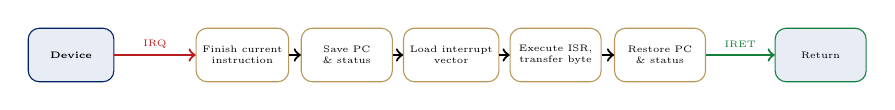
\begin{tikzpicture}[scale=0.68, transform shape,
          every node/.style={font=\tiny}]
      \node[draw=primary-blue, fill=light-bg, rounded corners,
            minimum width=1.6cm, minimum height=1.0cm, align=center]
            (DEV) at (0,0) {\textbf{Device}};
      \node[draw=primary-gold, fill=white, rounded corners,
            minimum width=1.7cm, minimum height=1.0cm, align=center]
            (Finish) at (3.2,0) {Finish current\\instruction};
      \node[draw=primary-gold, fill=white, rounded corners,
            minimum width=1.7cm, minimum height=1.0cm, align=center]
            (Save) at (5.15,0) {Save PC\\\& status};
      \node[draw=primary-gold, fill=white, rounded corners,
            minimum width=1.7cm, minimum height=1.0cm, align=center]
            (Vector) at (7.1,0) {Load interrupt\\vector};
      \node[draw=primary-gold, fill=white, rounded corners,
            minimum width=1.7cm, minimum height=1.0cm, align=center]
            (ISR) at (9.05,0) {Execute ISR,\\transfer byte};
      \node[draw=primary-gold, fill=white, rounded corners,
            minimum width=1.7cm, minimum height=1.0cm, align=center]
            (Restore) at (11.0,0) {Restore PC\\\& status};
      \draw[->, thick, negative] (DEV.east) -- node[above, negative,
        font=\tiny] {IRQ} (Finish.west);
      \draw[->, thick] (Finish.east) -- (Save.west);
      \draw[->, thick] (Save.east) -- (Vector.west);
      \draw[->, thick] (Vector.east) -- (ISR.west);
      \draw[->, thick] (ISR.east) -- (Restore.west);
      \node[draw=positive, fill=light-bg, rounded corners,
            minimum width=1.7cm, minimum height=1.0cm, align=center]
            (RET) at (14.0,0) {Return};
      \draw[->, thick, positive] (Restore.east) -- node[above, positive,
        font=\tiny] {IRET} (RET.west);
    \end{tikzpicture}
  \end{center}
  Key detail: the CPU checks the IRQ line \emph{at the end of an instruction},
  never mid-instruction --- so the interrupted program is always resumed at a
  clean instruction boundary.
\end{frame}

\begin{frame}{How Does the CPU Know Where the ISR Is?}
  \begin{block}{Two mechanisms}
    \begin{itemize}
      \item \key{Non-vectored}: all devices jump to \emph{one} common ISR,
        which polls each device to find the requester. Simple, but the search
        adds delay.
      \item \key{Vectored}: the device supplies an \key{interrupt vector}
        (an index/address of its own ISR) over the bus; the CPU uses it as an
        entry into the \key{interrupt vector table (IVT)}, jumping straight to
        the right routine.
    \end{itemize}
  \end{block}
  Vectored interrupts are why a fast device can get serviced with just a few
  extra cycles per interrupt --- the device hands the CPU its own branch
  address.
\end{frame}

\begin{frame}{Worked Example: Interrupt Overhead per Byte}
  \begin{exampleblock}{Cost arithmetic (keyboard resume)}
    One keystroke (100~ms apart) now costs: 1 instruction's finish, save
    PC/status ($\approx$ 10--50 cycles), jump via IVT, ISR + transfer
    ($\approx$ 30--50 cycles), restore and IRET ($\approx$10--20 cycles).
    \emph{Total: a few hundred cycles per \emph{byte}}, versus $10^8$ cycles
    for polling. The CPU keeps the other $\approx$99.99\% of the 100~ms.
  \end{exampleblock}
  \begin{itemize}
    \item \good{Interrupt-driven I/O turns waiting time into work.}
    \item \bad{But every interrupt still costs a save/restore + jump}: if a
      device interrupts too often (a disk at megabytes/s, byte at a time), the
      CPU drowns in \emph{overhead} rather than waiting. That motivates DMA
      (Act 4).
  \end{itemize}
\end{frame}

\begin{frame}{Priorities Among Devices: Who Interrupts First?}
  \begin{block}{Interrupt priority}
    When several devices interrupt at once, a priority scheme must pick one.
    Two classic implementations:
    \begin{itemize}
      \item \key{Daisy chain}: devices share one IRQ; the acknowledge signal
        ripples from highest-priority to lowest, and the first device that
        needs service grabs it --- giving \emph{non-uniform} priority by
        wiring position.
      \item \key{Multiple priority levels}: each level has its own IRQ line;
        higher levels can preempt lower ones. Safety-oriented sources (e.g.\ a
        CPU temperature sensor) get the top level.
    \end{itemize}
  \end{block}
  Always assign highest priority to interrupts whose delay causes the most
  damage --- damage, not data rate, is the first criterion.
\end{frame}

\begin{frame}{Interrupt-Driven I/O: Trade-offs}
  \begin{block}{Overhead-conscious}
    \begin{itemize}
      \item \good{Pro}: CPU works between events --- the $10^8$-cycle waste of
        polling disappears for slow devices.
      \item \good{Pro}: handles irregular, asynchronous events naturally ---
        keypresses, packets, sensors.
      \item \bad{Con}: per-interrupt save/restore cost. At very high event
        rates the overhead dominates: billions of small transfers per second
        through an ISR is not sustainable.
      \item \bad{Con}: ISR priority/masking logic adds real hardware
        complexity.
    \end{itemize}
  \end{block}
\end{frame}

\transitionslide{But a disk delivers megabytes per second — interrupt-per-byte would drown the CPU in overhead. What if the transfer happened without the CPU per byte at all?}

% =============================================================================
% ACT 4 --- DIRECT MEMORY ACCESS (DMA)
% =============================================================================
\section{Direct Memory Access (DMA)}

\begin{frame}{The Third Answer: DMA}
  \begin{block}{Direct memory access}
    A \key{DMA controller (DMAC)} is a dedicated hardware agent that
    transfers whole blocks \emph{device $\leftrightarrow$ memory} while the CPU
    does other work. The CPU \emph{programs} the DMAC once (device address,
    memory address, word count, direction), then the DMAC moves the block and
    raises \emph{one} interrupt when the whole block is done.
  \end{block}
  \begin{itemize}
    \item Compare Act 3: interrupts cost per \emph{byte}; DMA costs per
      \emph{block}. One interrupt for 20~KB instead of 20,000.
    \item New notation: \key{DMAC}, \key{burst} (block) mode, \key{cycle
      stealing} (below) --- added to the registry.
  \end{itemize}
  \cite{Hamacher2002_computer_organization}
\end{frame}

\begin{frame}{The DMA Controller at Work}
  \begin{center}
    % Diagram: DMA block diagram. CPU and main memory sit together on the
    % system bus; DMAC bridges device + DMAC registers (address, count,
    % control) to the same bus; DMAC signals CPU via DONE/IRQ. Bus takeover
    % arrows from DMAC to bus, interrupt from DMAC back to CPU.
    % Coordinates: (x, y)
    %   CPU at (0, 1.6); Memory at (0, -1.6); DMAC at (7, 0);
    %   Device at (11.4, 0)
    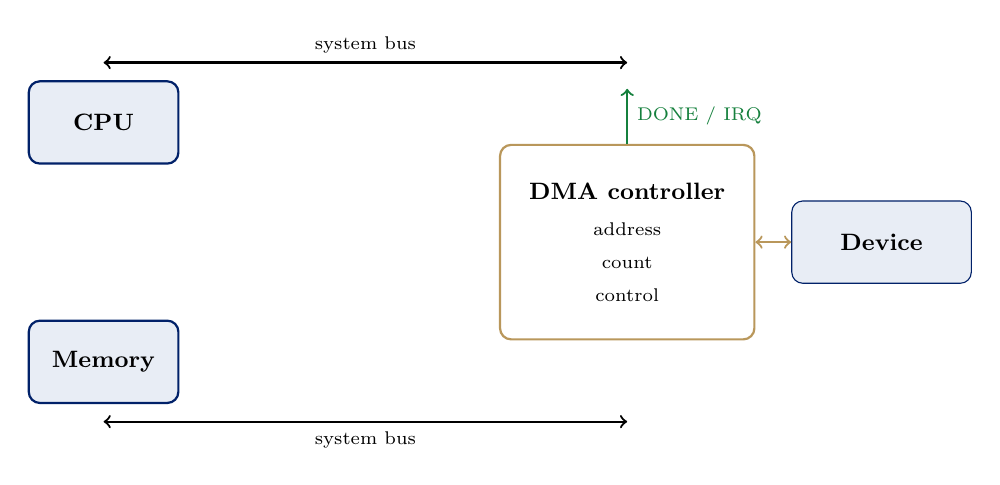
\begin{tikzpicture}[scale=0.95, transform shape,
        every node/.style={font=\small}]
      \node[draw=primary-blue, thick, fill=light-bg, rounded corners,
            minimum width=2.0cm, minimum height=1.1cm, align=center]
            (CPU) at (0,1.6) {\textbf{CPU}};
      \node[draw=primary-blue, thick, fill=light-bg, rounded corners,
            minimum width=2.0cm, minimum height=1.1cm, align=center]
            (MEM) at (0,-1.6) {\textbf{Memory}};
      \node[draw=primary-gold, thick, fill=white, rounded corners,
            minimum width=3.4cm, minimum height=2.6cm, align=center]
            (DMAC) at (7,0) {\textbf{DMA controller}\\[0.1cm]
            \scriptsize address\\[0.05cm]\scriptsize count\\[0.05cm]
            \scriptsize control};
      \draw[<->, thick] (CPU.north |- 0,2.4) -- (DMAC.north |- 0,2.4)
        node[midway, above, font=\scriptsize] {system bus};
      \draw[<->, thick] (MEM.south |- 0,-2.4) -- (DMAC.south |- 0,-2.4)
        node[midway, below, font=\scriptsize] {system bus};
      \node[draw=primary-blue, fill=light-bg, rounded corners,
            minimum width=2.4cm, minimum height=1.1cm, align=center]
            (DEV) at (10.4,0) {\textbf{Device}};
      \draw[<->, thick, primary-gold] (DMAC.east) -- (DEV.west);
      % DONE/IRQ arrow stops 0.35 short of the bus line (y=2.05, not 2.4) so
      % its up-pointing head does not coincide with the bus arrow's own
      % right-pointing head at (7, 2.4) --- see tikz-measurement.md Pass 4.
      \draw[->, thick, positive] (DMAC.north) -- node[right, positive,
        font=\scriptsize] {DONE / IRQ} (DMAC.north |- 0,2.05);
    \end{tikzpicture}
  \end{center}
  For the transfer, the DMAC becomes \key{bus master} --- it drives the bus
  itself, reading from the device and writing to memory (or vice versa) in
  bus-width chunks \cite{Hamacher2002_computer_organization}.
\end{frame}

\begin{frame}{DMA Modes: Burst vs.\ Cycle Stealing}
  \begin{block}{How the DMAC shares the bus}
    \begin{itemize}
      \item \key{Burst (block) mode}: the DMAC hogs the bus and transfers the
        whole block in one uninterrupted run --- highest throughput, but the
        CPU is shut out of the bus for the block's duration.
      \item \key{Cycle stealing}: the DMAC transfers one word each time the
        CPU would otherwise not use the bus (e.g.\ during an instruction's
        internal cycles), then releases --- the CPU barely notices, at the
        price of a slower block transfer.
      \item \key{Transparent mode}: transfers only while the CPU is guaranteed
        idle; lowest interference, lowest bandwidth.
    \end{itemize}
  \end{block}
  Block-transfer DMA with vectored interrupts maximizes raw I/O bandwidth.
\end{frame}

\begin{frame}{Worked Example: How Much CPU Does DMA Cost?}
  \begin{exampleblock}{Cost arithmetic}
    A 10~MB/s disk transfers 20~KB to memory by DMA. Processor runs at
    600~MHz and spends 300 + 900 = 1200 cycles total to \emph{initiate} and
    \emph{complete} the transfer. The block takes $20\text{ KB} / 10\text{
    MB/s} = 2$ ms; the processor does $600\!\times\!10^6 \times 2\!\times\!10^{-3}
    = 1.2\!\times\!10^6$ cycles in that time.
  \end{exampleblock}
  \[
    \text{CPU time consumed} = \frac{1200}{1.2\times 10^6}
    \times 100\% = 0.1\%.
  \]
  \begin{itemize}
    \item One interrupt at the end --- versus 20,000 in interrupt-driven byte
      mode. \good{DMA owns the block; the CPU pays a flat 0.1\%.}
  \end{itemize}
\end{frame}

\begin{frame}{DMA: Trade-offs}
  \begin{block}{Throughput vs.\ system-bus politics}
    \begin{itemize}
      \item \good{Pro}: bytes move at memory speed without per-byte CPU
        action --- this is how disks, networks, and GPUs actually ship data.
      \item \good{Pro}: single completion interrupt per block.
      \item \bad{Con}: the DMAC must arbitrate for the bus; during burst
        transfers the CPU's own memory access is delayed (the ``cycle
        stealing'' tension).
      \item \bad{Con}: setup + teardown overhead and real silicon --- you do
        not bolt DMA onto a single keyboard.
    \end{itemize}
  \end{block}
\end{frame}

\transitionslide{But DMA still needs the CPU to set up every transfer. What if an entire I/O program could run on its own processor?}

% =============================================================================
% ACT 5 --- I/O PROCESSORS AND SYNTHESIS
% =============================================================================
\section{I/O Processors and Synthesis}

\begin{frame}{The Fourth Answer: I/O Processor (IOP)}
  \begin{block}{I/O processor (I/O channel)}
    A small processor, capable of executing \key{I/O programs}, that manages
    transfers for \emph{many} devices. The CPU issues one high-level command
    (\texttt{start I/O on device \#7, block \#3}); the IOP runs a stored
    program --- issuing device commands, checking status, formatting data ---
    entirely off the main CPU's datapath.
  \end{block}
  \begin{itemize}
    \item \key{Selector channel}: controls several high-speed devices, but is
      dedicated to \emph{one} of them at a time until its transfer finishes.
    \item \key{Multiplexor channel}: interleaves data from \emph{several}
      slower devices at once, instead of finishing one before starting the
      next.
    \item DMA is \emph{fixed-function}; an IOP is \emph{programmed} --- its
      CPU cost drops to a few setup instructions per \emph{job}, not per byte
      or block.
  \end{itemize}
  \cite{Stallings2015_computer_organization}
\end{frame}

\begin{frame}{DMA vs.\ IOP, and the Four Techniques Head to Head}
  \footnotesize
  \resizebox{\textwidth}{!}{%
  \begin{tabular}{@{}lcccc@{}}
    \toprule
    & \textbf{Polling} & \textbf{Interrupt} & \textbf{DMA} & \textbf{IOP} \\
    \midrule
    CPU pays & every byte, in a loop & per event & per  block & per job \\
    Typical data rate & very low & low--medium & high & very high \\
    Extra hardware & none & IRQ/IVT logic & DMAC & a whole processor \\
    Best for & one simple, fast device & irregular async events & bulk
      transfers & many/varied devices \\
    \bottomrule
  \end{tabular}%
  }
  \vspace{0.3cm}
  \key{One clean rule of thumb}: polling for a dedicated always-nearly-ready
  device; interrupts for irregular events; DMA for bulk blocks; IOP when there
  is so much I/O that a whole processor is cheaper than babysitting transfers.
\end{frame}

\begin{frame}{Socratic Check: Which Technique, When?}
  \begin{columns}[T]
    \begin{column}{0.48\textwidth}
      \begin{alertblock}{Device droppings to classify}
        \begin{itemize}
          \item A keyboard, key pressed occasionally.
          \item A disk shipping 20~KB blocks at 10~MB/s.
          \item A memory-mapped sensor that is ready every microsecond.
          \item A RAID cabinet running many disks.
        \end{itemize}
      \end{alertblock}
    \end{column}
    \begin{column}{0.48\textwidth}
      \begin{block}{Arguments, concept by concept}
        \begin{itemize}
          \item Keyboard: \key{interrupt} --- irregular, long idle gaps.
          \item Disk: \key{DMA} --- one interrupt per block, not per byte.
          \item Sensor: \key{polling} --- always nearly ready, poll cost tiny.
          \item RAID: \key{IOP} --- a per-disk protocol machine is worth it.
        \end{itemize}
      \end{block}
    \end{column}
  \end{columns}
\end{frame}

\begin{frame}{The Thread Concludes: Cost per Byte, Four Ways}
  \footnotesize
  \begin{tabular}{@{}lcl@{}}
    \toprule
    \textbf{Technique} & \textbf{CPU cost} & \textbf{Why} \\
    \midrule
    Polling (keyboard byte) & $\sim 10^8$ cycles & endless busy-wait \\
    Interrupt (keyboard byte) & $\sim 10^2$--$10^3$ cycles & one save/restore +
      ISR \\
    DMA (20~KB disk block) & 1200 cycles / block & flat setup + 1 interrupt \\
    IOP (whole disk job) & a few setup instructions & runs its own program \\
    \bottomrule
  \end{tabular}
  \vspace{0.3cm}
  \begin{alertblock}{The one-sentence takeaway}
    Every technique moves the same bytes; they differ in \emph{how many CPU
    cycles are spent per byte moved} --- polling spends the most, the IOP the
    least --- and you should select the cheapest one that still gets the bytes
    there in time (the Week 8 learning objective).
  \end{alertblock}
\end{frame}

\begin{frame}{Bridge to Week 9}
  \begin{exampleblock}{From moving data to keeping it}
    This week moved bytes from the outside world \emph{into memory}. Week 9
    asks how memory itself is organized --- caches, the memory hierarchy, and
    which bytes are worth keeping close. The DMA block you just moved lands in
    that hierarchy.
  \end{exampleblock}
  \begin{itemize}
    \item The throughput you defend with a technique is bounded by the memory
      system it feeds --- DMA is only as fast as main memory allows.
    \item Next week's cache question is: \emph{given} a memory you cannot make
      uniformly fast, where does the data go?
  \end{itemize}
\end{frame}

\begin{frame}{Summary}
  \begin{itemize}
    \item \key{Synchronous} I/O assumes fixed timing; \key{asynchronous} I/O
      handshakes per transfer (\emph{DATA READY}/\emph{ACKNOWLEDGE}) --- the
      only sane way to talk to devices of wildly different speeds.
    \item \key{Polling} is simplest and cheapest in hardware but wastes the
      most CPU ($10^8$ cycles/keypress in our example).
    \item \key{Interrupt-driven I/O} releases the CPU between events and drops
      the per-byte cost to a few hundred cycles --- at the price of ISR /
      priority hardware.
    \item \key{DMA} moves whole blocks with one completion interrupt --- 0.1\%
      CPU in the worked example above; choose \key{burst} for throughput and
      \key{cycle stealing} for CPU friendliness.
    \item \key{IOP} is a programmable processor for whole I/O jobs.
    \item \key{Select on cost per byte vs.\ latency/throughput} --- never on
      habit.
  \end{itemize}
\end{frame}

\begin{frame}{References}
  \footnotesize
  \bibliographystyle{plain}
  \bibliography{../../Bibliography_base}
\end{frame}

\end{document}
